\documentclass[a4paper,american,10pt]{paper}
\usepackage[T1]{fontenc}
\usepackage[utf8]{inputenc}
\pagestyle{plain}
\usepackage{babel}
\usepackage{textcomp}
\usepackage[mathscr]{euscript}
\usepackage{amsmath}
\usepackage{amsthm}
\usepackage{setspace}
\usepackage[unicode=true]{hyperref}
\usepackage{breakurl}
\usepackage{txfonts}
\usepackage{pxfonts}
\usepackage{tikz}
\usetikzlibrary{arrows.meta,positioning,calc}
\usepackage{tkz-graph}
\usepackage{algorithm}
\usepackage{algpseudocode}
\usepackage{graphicx}
\usepackage{float}
\usepackage{needspace}
\usepackage[left=3.5cm,right=3.5cm]{geometry}
\usepackage{wasysym}
\usepackage{subcaption}
\usepackage{mdframed} % Add easy frames to paragraphs
\usepackage{lipsum} % For dummy text
\usepackage{xcolor}
\usepackage{xparse} % Add support for \NewDocumentEnvironment

\graphicspath{ {./images/} }
\date{\today}

% >-> Overset Arrow
\makeatletter
\newbox\xrat@below
\newbox\xrat@above
\newcommand{\xrightarrowsingletail}[2][]{%
  \setbox\xrat@below=\hbox{\ensuremath{\scriptstyle #1}}%
  \setbox\xrat@above=\hbox{\ensuremath{\scriptstyle #2}}%
  \pgfmathsetlengthmacro{\xrat@len}{max(\wd\xrat@below,\wd\xrat@above)+.6em}%
  \mathrel{\tikz [>->,baseline=-.75ex]
                 \draw (0,0) -- node[below=-2pt] {\box\xrat@below}
                                node[above=-1pt] {\box\xrat@above}
                       (\xrat@len,0) ;}}
\makeatother

% >-> Arrow
\makeatletter
\newbox\xrat@below
\newbox\xrat@above
\newcommand{\rightarrowsingletail}[2][]{%
  \setbox\xrat@below=\hbox{\ensuremath{\scriptstyle #1}}%
  \setbox\xrat@above=\hbox{\ensuremath{\scriptstyle #2}}%
  \pgfmathsetlengthmacro{\xrat@len}{max(\wd\xrat@below,\wd\xrat@above)+.6em}%
  \mathrel{\tikz [>->,baseline=-.75ex]
                 \draw (0,0) -- node[below=-2pt] {\box\xrat@below}
                                node[above=-1pt] {\box\xrat@above}
                       (0.5,0) ;}}
\makeatother

% >>-> Overset Arrow
\makeatletter
\newbox\xrat@below
\newbox\xrat@above
\newcommand{\xrightarrowdoubletail}[2][]{%
  \setbox\xrat@below=\hbox{\ensuremath{\scriptstyle #1}}%
  \setbox\xrat@above=\hbox{\ensuremath{\scriptstyle #2}}%
  \pgfmathsetlengthmacro{\xrat@len}{max(\wd\xrat@below,\wd\xrat@above)+.6em}%
  \mathrel{\tikz [>>->,baseline=-.75ex]
                 \draw (0,0) -- node[below=-2pt] {\box\xrat@below}
                                node[above=-1pt] {\box\xrat@above}
                       (\xrat@len,0) ;}}
\makeatother

% >>-> Arrow
\makeatletter
\newbox\xrat@below
\newbox\xrat@above
\newcommand{\rightarrowdoubletail}[2][]{%
  \setbox\xrat@below=\hbox{\ensuremath{\scriptstyle #1}}%
  \setbox\xrat@above=\hbox{\ensuremath{\scriptstyle #2}}%
  \pgfmathsetlengthmacro{\xrat@len}{max(\wd\xrat@below,\wd\xrat@above)+.6em}%
  \mathrel{\tikz [>>->,baseline=-.75ex]
                 \draw (0,0) -- node[below=-2pt] {\box\xrat@below}
                                node[above=-1pt] {\box\xrat@above}
                       (0.5,0) ;}}
\makeatother

\makeatletter
\providecommand*{\code}[1]{\texttt{#1}}
\makeatother

\newtheorem{thm}{Theorem}

\renewcommand{\algorithmicrequire}{\textbf{Input:}}
\renewcommand{\algorithmicensure}{\textbf{Output:}}
\algnewcommand{\TRUE}{\textbf{true}}
\algnewcommand{\FALSE}{\textbf{false}}

\counterwithin*{equation}{section}
\counterwithin*{equation}{subsection}

\theoremstyle{definition}\newtheorem{definition}{Definition}
\hyphenation{counterfactual}
\hyphenation{possible}
\hyphenation{worlds}
\hyphenation{model}
\hyphenation{structure}

% Example environment
\definecolor{graylight}{cmyk}{.30,0,0,.67} % define color using xcolor syntax
\newmdenv[ % Define mdframe settings and store as leftrule
  linecolor=graylight,
  topline=false,
  bottomline=false,
  rightline=false,
  skipabove=\topsep,
  skipbelow=\topsep
]{leftrule}

\NewDocumentEnvironment{examplef}{O{\textbf{Example:}}} % Define example environment
{\begin{leftrule}\noindent\textcolor{graylight}{#1}\par}
{\end{leftrule}}

% Consideration environment
\NewDocumentEnvironment{consider}{O{\textbf{Consider:}}} % Define consideration environment
{\begin{leftrule}\noindent\textcolor{graylight}{#1}\par}
{\end{leftrule}}



\begin{document}

\title{An interactive demonstration of counterfactual truth conditions}

\subtitle{Bachelor Thesis}

\author{%
	Andreas Paul Bruno Lönne\\
	\code{\href{mailto:loenne@campus.tu-berlin.de}{loenne@campus.tu-berlin.de}}
}

\institution{
	Technische Universität Berlin\\
	Degree program: Bachelor Informatik / Computer Science
}

\maketitle

\begin{abstract}
In this thesis, I address the scarcity of online resources showcasing Lewis' counterfactual truth conditions in an intuitive and digestible manner. To this end, I (i) formulate a semantic reachability game for counterfactual sentences; (ii) prove that it always halts after a finite number of moves; (iii)~prove its correctness and (iv) develop a browser-based web-application to showcase the semantic game of counterfactuals.
\end{abstract}
\section{Introduction}
Counterfactuals are a contentious subject of ongoing philosophical and mathematical discourse. The insufficiencies of truth-functional treatments of counterfactuals, sparked a plethora of models giving alternate accounts of counterfactual truth conditions. One of the more well known and controversial attempts to do so is David K. Lewis' formulation of the counterfactual operators $\boxright$ and $\Diamondright$. But despite its prominence there are few resources to introduce Lewis' interpretation of counterfactuals as variably strict conditionals.\\

- set out to create an interactive demonstration of lewis counterfactual truth conditions\\
- Can be found under Github Link\\
- But first introduce counterfactuals ...\\
A\\\\\\\\\\\\\\\\\\\\\\\\\\\\\\\\\\\\\\\\
In this thesis I make the attempt to create an application that is able to convey Lewis' counterfactual truth conditions by way of a semantic two-player game and inspire players to learn more about counterfactuals.\\
\textit{Background and literature\\
- contentious subject within philosophy (Lewis realism about possible worlds (Are possible worlds real?) and comparative similarity (Can you weigh differences up against each other?))
- academic standstill for about 50 years
- you can find this demo under ... on github
To this end i defined a semantic game of counterfactuals and implemented a browser-based demonstration game.\\
The document is laid out as follows:\\
First i will explain counterfactuals.\\
First i will begin by introducing the counterfactual logic I am basing the semantic game of counterfactuals on. Then i will give game-theoretical definitions and formulate two versions of the semantic game. After that ...}
\section{Counterfactuals}
\textit{Counterfactuals} are statements about what might or would have been the case, if things took place differently than they did. One may think to themselves "If I had not forgotten about my appointment, I would have been punctual". Or one may wonder "If Alexander the Great had not died at the age of 32 and attacked Europe, would the Romans have defeated him?". Such \textit{counterfactual~thought}---that is the thought of alternate outcomes---is essential for reasoning, deduction and cognitive function. \cite{byrne_counterfactual_2016} Due to its abundance in human thought, the ability to imagine alternate realities seems trivial to most. But making rigorous statements or claims about them is difficult. This is because communicating a complete and consistent account of the state of affairs of an alternate reality---similar in complexity to ours--- is difficult, if not impossible. One may attempt to circumvent this issue by giving the state of affairs of an alternate reality as a deviation from the state of affairs of reality. But consider this. 
Take our previous example about Alexander the Great and assume that the imagined alternate reality is identical to our reality, except that Alexander the Great did not die at the age of 32 and attacked Europe. Now suppose we know about reality, that Alexanders troops remained outside of Europe. Then this should also be the case in the alternate reality we attempted to describe. If we are to assume that an army cannot be in two places at the same time and Alexander could not have attacked Europe without his army, then Alexanders troops could not have remained outside of Europe and attacked Europe at the same time.
We find, that simply deviating from our own reality in a few concrete ways may produce internally inconsistent alternate realities, which cannot be alternate realities, because they are not ways the world could have been.\\
To avoid this problem we forgo describing alternate realities all-together. We call a complete and consistent way the world is or could have been, a possible world. And agree that we refer to a possible world, most similar to ours, where our stipulation is true. So our example is to be read as "In a world most similar to our own, where Alexander the Great did not die at the age of 32 and attacked Europe, the Romans would have defeated him". In this way---although we may not know the state of affairs of a possible world---we are able to assign definite truth values to our counterfactual sentence for any possible state of affairs at that world. However we need to note, that this approach assumes the notion of comparative similarity between possible worlds. Which means that given any 3 worlds $w,v_1,v_2$, with respect to their overall similarity from the standpoint of $w$, either
\begin{itemize}
\item $w$ is more similar to $v_1$, than to $v_2$,
\item $w$ is more similar to $v_2$, than to $v_1$,
\item or $w$ is equally similar to $v_1$ and $v_2$.
\end{itemize}
While the notion of an aggregate overall similarity between possible worlds appears justified at first glance, it has been subject of contention. \cite{morreau_overall_similarity_2010}
\section{Lewis' counterfactual operators}
With these introductory thoughts out of the way, let us talk in greater detail about the counterfactual operators themselves. Lewis introduces the counterfactual would $\boxright$ and counterfactual might $\Diamondright$ operators as binary modal operators. \cite{lewis_counterfactuals_1973} When we write $\varphi\boxright\psi$, we call the formula $\varphi$ the antecedent and the formula $\psi$ the consequent. We may informally rewrite one of our former examples as "I~did~not~forget~about~my~appointment~$\boxright$~I~was~punctual" and read it the following way. Read $\varphi\boxright\psi$ as "If it were the~case that $\varphi$, then it would be the case that $\psi$", and read $\varphi\Diamondright\psi$ as "If it were the case that~$\varphi$, then~it might be the case that $\psi$". We further dedicate the remainder of this section to summarizing and explaining Lewis' truth conditions for $\boxright$ and $\Diamondright$.\\
\subsection{Lewis' system of spheres}
The truth conditions of the counterfactual operators are stated with respect to a structure, called a \textit{system~of~spheres}. Lewis defines a system~of~spheres as follows.
\begin{definition}[Lewis' system of spheres]
Let $\$$ be an assignment to each possible world $i$ of a set $\$_i$ of sets of possible worlds. Then $\$$ is called a (centered) system of spheres, and the members of each $\$_i$ are called spheres around $i$, if and only if, for each world $i$, the following conditions hold.
	\begin{itemize}
	\item[(C)] $\$_i$ is centered on $i$; that is, the set $\{i\}$ having $i$ as its only member belongs to $\$_i$.
	\item[(1)] $\$_i$ is nested; that is, whenever $S$ and $T$ belong to $\$_i$, either $S$ is included in $T$ or $T$ is included in $S$.
	\item[(2)] $\$_i$ is closed under unions; that is, whenever $\mathscr{S}$ is a subset of $\$_i$ and $\bigcup\mathscr{S}$ is the set of all worlds $j$ such that $j$ belongs to some member of $\mathscr{S}$, $\bigcup\mathscr{S}$ belongs to $\$_i$.
	\item[(3)] $\$_i$ is closed under (nonempty) intersections; that is, whenever $\mathscr{S}$ is a nonempty subset of $\$_i$ and $\bigcap\mathscr{S}$ is the set of all worlds $j$ such that $j$ belongs to every member of $\mathscr{S}$, $\bigcap\mathscr{S}$ belongs to $\$_i$.
	\end{itemize}
	\label{def:system_of_spheres}
\end{definition}
\noindent Now let us first take a broad perspective upon this definition. Most generally a system of spheres is an assignment of a set of sets of possible worlds to each world. The assigned sets exhibit the four characteristics (C), (1), (2) and (3); and are called sets of spheres. In totality such a system of spheres serves to codify the relationships of accessibility and comparative~similarity between possible worlds. To this end each set of spheres describes an ordering of possible worlds with respect to similarity to the world it is assigned to. Meaning, that the set of spheres $\$_i$ describes the comparative~similarity to- and accessibility from $i$ for each world. This is briefly illustrated by the next example.

\begin{figure}[H]
\centering
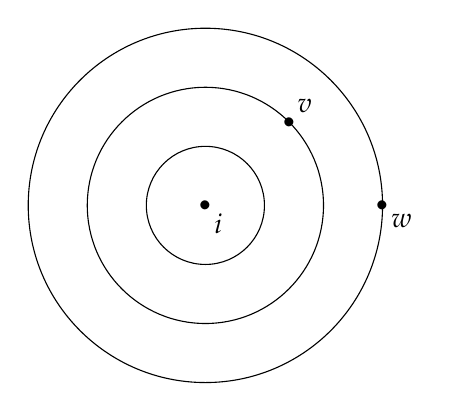
\begin{tikzpicture}[
roundnode/.style={circle, draw=black!0, fill=black!100, very thick, minimum size=1pt},
]
\coordinate (O) at (0,0);
\coordinate (V) at (45:1.5);
\coordinate (W) at (0:2.25);
\draw (O) circle (2.25);
\draw (O) circle (1.5);
\draw (O) circle (0.75);
\node[scale=1mm, label={[label distance=-6mm]315:$i$}] at (O) {.};
\node[scale=1mm, label={[label distance=-6mm]45:$v$}] at (V) {.};
\node[scale=1mm, label={[label distance=-6mm]315:$w$}] at (W) {.};

%\draw[black] (0,0) -- (1,0);
\end{tikzpicture}
\caption{A set of spheres $\$_i=\{\{ i\} ,\{ i,v\} ,\{ i,v,w\}\}$}
\label{fig:set_of_spheres}
\end{figure}

\noindent In this example we look at the worlds $i$, $v$ and $w$; and consider the set of spheres $\$_i$. The spheres themselves are sets of possible worlds and are visualized through circles. A world inside or on the circumference of a circle is contained within the corresponding sphere. Crucially, the meaning of a sphere around $i$ is that each world contained in it is more similar to $i$ than each world not contained in it. For our example this means that $i$ is more similar to itself than any other world; $i$ and $v$ are more similar to $i$ than any other world; and that $i$, $v$ and $w$ are more similar to $i$ than any other world. Regarding accessibility, a world is said to be accessible from $i$, if it is contained in any sphere around $i$. So we can see that all $i$, $v$ and $w$ are accessible from $i$. With this in mind, we can motivate the properties (C), (1), (2) and (3).\\

(C) It seems reasonable to assume that each world is most similar to itself and that there cannot be another world equally or more similar to it than itself. If that is the case, every sphere around a world $i$ needs to contain the set $\{ i\}$.\\
\indent (1) Intuitively it may also make sense, that for each pair of spheres around the same world one should include the other. If we entertain the notion, that the spheres around a world are not nested, then one of those spheres cannot be a sphere. First, remember that a sphere around a world $i$ is a set of possible worlds, such that each world contained in it is more similar to $i$, than every world not contained in it. Then suppose the set of spheres $\$_i$ is not nested. In that case two worlds $v$ and $w$ and the spheres $S,T\in\$_i$ exist, such that $v\in S$, $w\notin S$, $v\notin T$ and $w\in T$. Through $S$ we know that that $v$ is more similar to $i$ than $w$. And through $T$ we know that that $w$ is more similar to $i$ than $v$. Which cannot both be the case at the same time.\\
\indent (2) Suppose that for the union $\bigcup\mathscr{S}$ of a set of spheres $\mathscr{S}$ around $i$, there are two worlds $v,w$ such that $v\in\bigcup\mathscr{S}$ and $w\notin\bigcup\mathscr{S}$. Then that means, that $v$ is, and $w$ is not, contained in some sphere in $\mathscr{S}$. Hence $v$ is more similar to $i$ than $w$. Therefore $\bigcup\mathscr{S}$ is a set such that any world contained within it is more similar to $i$ than any world not contained in it. We call such a set a sphere around $i$.\\
\indent (3) Suppose that for the intersection $\bigcap\mathscr{S}$ of a nonempty set of spheres $\mathscr{S}$ around $i$, there are two worlds $v,w$ such that $v\in\bigcap\mathscr{S}$ and $w\notin\bigcap\mathscr{S}$. Then that means, that $v$ is, and $w$ is not, contained in some sphere in $\mathscr{S}$. Hence $v$ is more similar to $i$ than $w$. Therefore $\bigcap\mathscr{S}$ is a set such that any world contained within it is more similar to $i$ than any world not contained in it. We call such a set a sphere around $i$.
\subsection{Lewis' counterfactual truth conditions}
Then let us take a look at Lewis' counterfactual truth conditions. Take the counterfactual operators as part of some logic, where formulas like $\varphi$ and $\psi$ are evaluated with respect to some world and a system of spheres. Lewis abbreviates a world, where the formula $\varphi$ holds as a $\varphi$-world. The truth conditions of Lewis' counterfactual would operator are these.
\begin{definition}[Counterfactual would]
	$\varphi\boxright\psi$ is true at a world i (according to a system of spheres \$) if and only if either
	\begin{itemize}
	\item[(1)] no $\varphi$-world belongs to any sphere $S$ in $\$_i$, or
	\item[(2)] some sphere $S$ in $\$_i$ does contain at least one $\varphi$-world, and $\varphi\rightarrow\psi$ holds at every world in $S$.
	\end{itemize}
	%\caption{Lewis' counterfactual would truth conditions}
	\label{def:counterfactual_would}
\end{definition}
\noindent The counterfactual would evaluates to true iff either (1) or (2) is true.\\
\indent (1) We describe the first case as vacuous truth. Intuit this case the same way a material implication is true, when its antecedent is false. From wrong antecedents arbitrary consequents may be inferred. Keep in mind however, that the vacuous truth of the counterfactual would is much stricter. While the material conditional only requires the antecedent to be false at the world it is evaluated at, the counterfactual would requires the antecedent to be false at every accessible world.\\
\indent (2) The non-vacuous case requires the existence of a sphere throughout which $\varphi\rightarrow\psi$ holds and that that sphere also contains a $\varphi$-world. The existence of such a sphere can roughly be understood as the existence of some accessibility restriction under which the strict conditional $\Box (\varphi\rightarrow\psi)$ comes out as non-vacuously true. Meaning that $\varphi\rightarrow\psi$ holds throughout all accessible worlds and that at least one accessible world is a $\varphi$-world. While the strict conditional is true, only if it is true in the broadest sense---meaning it is true at every accessible world---the counterfactual would conditional merely needs to be true in one of many senses. That is why Lewis' counterfactual operators are called variably strict conditionals. Each of these many senses are degrees of similarity to a world, that are described by spheres around that world. To motivate why overall similarity between worlds is used as an accessibility restriction consider this example.
\begin{equation}
\text{"If Kennedy had pressed the red button, there would have been nuclear war"}
\end{equation}
We consider this to be true. Without much trouble, one can make up many counterexamples to this counterfactual. Imagine for a moment the possibility that Kennedy had pressed the red button and the button malfunctioned. In that case Kennedy pressed the button, but there is no nuclear war. Obviously that is not meant. When we say something like "If~it~were~the~case that A, then it would be the case that B", we implicitly mean "If it were the case that~A and things were pretty much as they are otherwise, then it would be the case that~B". Our rebuttal therefore may be that there is at least one possible world where Kennedy pressed the red button and the red button did not malfunction that is more similar to the actual world than any possible world where Kennedy pressed the red button and the button did malfunction. If this is the case, we may claim that our example counterfactual is true, although there are certain senses in which it is not true. This is why a counterfactual would operator is true, if there is at least one sense, represented through a sphere of accessibility, in which it is true. Regarding the system of spheres it means that a counterfactual would operator is non-vacuously true, unless each sphere around the world it is evaluated at contains a refuting world that serves as a counterexample or no sphere around the world it is evaluated at contains a $\varphi$-world.\\
The \textit{counterfactual~might} is defined analogously.

\begin{definition}[Counterfactual might]
	$\varphi\Diamondright\psi$ is true at a world i (according to a system of spheres \$) if and only if both
	\begin{itemize}
	\item[(1)] some $\varphi$-world belongs to some sphere $S$ in $\$_i$, and
	\item[(2)] every sphere $S$ in $\$_i$ that contains at least one $\varphi$-world contains at least one world where $\varphi\wedge\psi$ holds.
	\end{itemize}
	\label{def:counterfactual_might}
\end{definition}

\noindent Note the differences in quantification and truth conditions. The counterfactual would's existential quantifier for the existance of a sphere is replaced by a universal quantifier requiring every sphere containing a $\varphi$-world to also contain a $(\varphi\wedge\psi)$-world. While the counterfactual would requires each world of a sphere to fulfill its criteria, the counterfactual might requires one world of each sphere, that contains a $\varphi$-world, to fulfill its criteria. Notice also that the counterfactual might does not have two separate truth cases and is true in only one case. But since \cite{lewis_counterfactuals_1973} shows that the counterfactual would and counterfactual might are interdefinable as stated in equations \ref{eq:would_interdef} and \ref{eq:might_interdef}, we wont go into further detail here.
\begin{equation}
\label{eq:would_interdef}
\varphi\boxright\psi =^{def} \neg (\varphi\Diamondright\neg\psi )
\end{equation}
\begin{equation}
\label{eq:might_interdef}
\varphi\Diamondright\psi =^{def} \neg (\varphi\boxright\neg\psi )
\end{equation}

\section{Counterfactual logic}
This section is concerned with defining counterfactual logic. First it provides a brief definition of well-formed counterfactual formulas, then introduces the structure they are evaluated on and concludes by defining the truth conditions of counterfactual logic.

\subsection{Counterfactual formulas}
We call $\Phi = \{\varphi ,\psi ,...\}$ the set of all well-formed counterfactual formulas.
\begin{definition}[Well-formed counterfactual formula]
Given an infinite set of atomic formula symbols $Atoms = \{ x, y, ...\}$ and an alphabet $A~=~\{\bot ,\top ,\neg ,\vee ,\wedge ,\Diamond ,\Box ,\boxright ,\Diamondright\}\cup Atoms$, the structure of every well-formed counterfactual formula is expressed through the following Backus-Naur form.
\begin{equation}
\varphi, \psi ::= \bot \mid \top \mid x \mid \neg \varphi \mid \varphi \vee \psi \mid \varphi \wedge \psi \mid \Diamond \varphi \mid \Box \varphi \mid \varphi \boxright \psi \mid \varphi \Diamondright \psi
\end{equation}
\end{definition}

\subsection{Counterfactual~Kripke~structure}
In order to evaluate the non-truth-functional connectives of counterfactual~logic, we define a variation of the Kripke~structure in \cite{kripke_modal_logic_1963}. To evaluate Lewis' counterfactual truth conditions \cite{lewis_counterfactuals_1973}, we also introduce a notion of similarity between possible worlds to the accessibility relation.
\begin{definition}[counterfactual Kripke structure]
A {\it counterfactual Kripke structure} is an ordered triple $(W, \leadsto ,F)$, consisting of
\begin{itemize}
\item the set of all possible~worlds $W=\{w,v,...\}$,
\item the similarity relation $\leadsto$ with $\{(w,0,w)\mid w\in W\}\subseteq$ $\leadsto$ that contains up to one tuple $(w, r, w')$ with $r\in$ $]0,\infty]$ for each ordered pair of worlds $(w,w')\in W\times W$, and
\item an assignment of each world, to a set of atomic formulas $F \colon W \rightarrow 2^{Atoms}$.
\end{itemize}
To describe common accessiblity relationships between possible worlds more succinctly, we introduce the shorthands $W_w = \{w'\mid \smash{w \overset{r}{\leadsto} w'}\}$, $W_{w,r}^\leq = \{w'\mid \smash{w \overset{r'}{\leadsto} w'}\wedge r'\leq r\}$ and $W_{w,r}^< = \{w'\mid \smash{w \overset{r'}{\leadsto} w'}\wedge r'< r\}$.
\end{definition}
\noindent Let us explain further the members of our counterfactual~Kripke~structure.\\
The set of all possible~worlds $W$ represents all complete and self-consistent ways reality could have been. $F$ in turn, describes the state of affairs at each world. It assigns to each world a set of atomic propositions, that are the case at it. The similarity relations purpose is twofold. It serves as an accessibility relation, restricting accessibility between worlds and also carries information about comparative similarity between worlds. In particular this means for any two worlds $w$ and $v$, that iff $\smash{w\overset{r}{\leadsto}v}$, then $v$ is called accessible from $w$. $\smash{w\overset{r}{\leadsto}v}$ also means, that $r$ is a measure of similarity between $w$ and $v$, from the standpoint of $w$. We can suppose another world $v'$, with $\smash{w\overset{r'}{\leadsto}v'}$ and compare $r$ and $r'$. If $r < r'$, we can conclude, that $v$ is more similar to $w$ than $v'$, from the standpoint of $w$. Additionally we note, that for our purposes $\leadsto$ will contain a tuple $(w, 0, w)$ for each world $w\in W$. This is because we assume analogously to Kripke, that worlds are self-similar and are accessible from themselves.
%\newpage
\subsection{Truth conditions of counterfactual logic}
Given a counterfactual~Kripke~structure $S = (W, \leadsto ,F)$ and a world $w$,\\
$S,w\nvDash\bot$.\\
$S,w\vDash\top$.\\
$S,w\vDash x$ iff $x\in F(w)$.\\
$S,w\vDash \neg\varphi$ iff $S,w\nvDash\varphi$.\\
$S,w\vDash \varphi\vee\psi$ iff ($S,w\vDash\varphi$ or $S,w\vDash\psi$).\\
$S,w\vDash \varphi\wedge\psi$ iff ($S,w\vDash\varphi$ and $S,w\vDash\psi$).\\
$S,w\vDash \Diamond \varphi$ iff a world $w'\in W_w$ exists, such that $S,w' \vDash \varphi$.\\
$S,w\vDash \Box \varphi$ iff for every world $w'\in W_w$, it is true that $S,w' \vDash \varphi$.\\
$S,w \vDash \varphi \boxright \psi$, iff either
\begin{itemize}
	\item[(1)] no world $w'\in W_w$ exists, such that $S,w' \vDash \varphi$, or
	\item[(2)] a world $w'$ and an $r$ exist, such that $w\overset{r}{\leadsto} w'$ and $S,w'\vDash \varphi$ and for each world $w^*$, for which an $r^*$ exists, such that $r^*\leq r$ and $w\overset{r^*}{\leadsto} w^*$, it is true that $S,w^*\vDash\neg\varphi\vee\psi$.
\end{itemize}
\noindent$S,w\vDash \varphi \Diamondright \psi$, iff both 
\begin{itemize}
	\item[(1)] a world $w'\in W_w$ exists, such that $S,w' \vDash \varphi$, and
	\item[(2)] for every world $w''$, for which an $r''$ exists, such that $w\overset{r''}{\leadsto}w''$ and $S,w'' \vDash \varphi\wedge\neg\psi$ are true, a world $w^*$ and an $r^*$ exist, such that $r^* \leq r''$ and $w\overset{r^*}{\leadsto}w^*$ and $S,w^* \vDash \varphi\wedge\psi$.
\end{itemize}
\section{The semantic game of counterfactuals}
This section offers an overview and introduction to the semantic~game~of~counterfactuals. The semantic~game~of~counterfactuals is a sequential two-player reachability game, wherein a \textit{defender} $d$ tries to prove a counterfactual formula and an \textit{attacker} $a$ tries to disprove it. The defender begins the game as the \textit{active~player}, with a counterfactual~formula at a possible~world. The active player is a role assigned to the player that can currently make moves and whose typical objective it is to prove the current formula through play. As the active player makes moves, the counterfactual formula is resolved progressively until a player resolves a $\top$ and wins; or cannot make any move and loses. Throughout the game, moves may change the active player and current world.

\subsection{Definition of the semantic game}
The game itself is akin to a discussion where players make arguments and refute them. Weak arguments do not hold up to scrutiny, but strong ones do. The players' adversarial interplay allows the discovery and dismissal of arguments, such that the reason for truth or falsity of a claim is revealed. Let us begin by giving the definition of the semantic game and subsequently introduce its members.
\begin{definition}[Semantic game of counterfactuals]
The two formulations of the semantic game of counterfactuals $\mathfrak{T}[\varphi ,w,S]=(I, E, G, \rightarrowsingletail{})$ and $\mathfrak{G}[\varphi ,w,S]=(I, E, G, \rightarrowdoubletail{})$ with respect to a formula $\varphi\in\Phi$, a world $w\in W$ and a counterfactual Kripke structure $S=(W,\leadsto ,F)$ are ordered tuples, consisting of
\begin{itemize}
\item an initial game state $I=(\varphi ,w)_d$,
\item a set of winning game states $E=\{(\top ,w)_p \mid w\in W\wedge p\in\{ a,d\}\}$,
\item a set of all game states $G$, and
\item a transition relation $\rightarrowsingletail{}$ or $\rightarrowdoubletail{}$, depending on the formulation.
\end{itemize}
We employ the notation $\mathfrak{T}_p[\varphi ,w,S]$ or $\mathfrak{S}_p[\varphi ,w,S]$ that means that the annotated player $p\in\{a,d\}$ begins the game; that is, $I=(\varphi ,w)_p$ instead of $I=(\varphi ,w)_d$.
\end{definition}
The initial game state $I$ varies from game to game. It contains the formula $\varphi$ that ought to be proven and the world $w$ it ought to be proven at. It is always indexed by the initial active player, that is the defender. The set of winning game states contains all game states in which the active player wins. When the active player wins, the respective other player loses. The set $E$ includes all game states where the formula is resolved to a $\top$-symbol. It is also possible for a player to win without reaching a winning game state. This is the case when the active player is unable to make a move and is stuck. When this happens, the active player loses and the active player's opponent i.e. the inactive player wins. $\mathfrak{S}[\varphi ,w,S]$ also contains the set of all game states $G$ and the set of transitions between game states which we call the set of moves. In later sections we will define two such sets of moves. One general formulation $\rightarrowsingletail{}$ and another formulation $\rightarrowdoubletail{}$ employing the limit assumption. In order to arrive at our definition for $\rightarrowsingletail{}$ and $\rightarrowdoubletail{}$, let us first define game states and transitions.

\subsection{Game states}
Game states form the backbone of the semantic game of counterfactuals by describing its game positions. Each game state describes the game at a discrete point in time in-between moves.
\begin{definition}[Game states]
A game state $g\in G$ is a tuple that can take any one of the forms
\begin{itemize}
	\item[(1)] $(\varphi ,w)_p$
	\item[(2)] $(\varphi ,w, e)_p$
	\item[(3)] $(\varphi ,w,w',r)_p$
\end{itemize}
where $\varphi\in\Phi$; $w,w'\in W$; $r\in [0,\infty ]$ and $p,e\in\{ a,d\}$.
\end{definition}
\noindent Of these types of game states (1) is the most common. It carries a counterfactual formula, the current world and is indexed with the active player. It is employed to resolve atomic formulas $x,y,...$ and the propositional symbols $\top,\neg,\vee,\Diamond$; while also serving as an initial and final state type for other resolutions. (2) is a type of game state that represents a player temporarily becoming active and choosing a state transition. $e$ holds the previous active player, which will resume being active after the next state transition and differentiates this type of game state from (1). Lastly, game~state~type~(3) is an extension of~(1), describing a game state where a sphere~of~accessibility has been chosen. $w'$ is a \textit{sphere-delimiting~world}, lying exactly on the surface of said sphere~of~accessibility with radius $r$. We will look at this in further detail in the next subsection.\\

\subsection{Moves}
When the active player transforms the current game state into another and progresses the game, we call that a move. Formally we represent this through a tuple of game states.
\begin{definition}[Move]
A move $m$ is a tuple $m\in G\times G$.
\end{definition}
\noindent The first element of the tuple is the initial game state, while the second one is the resulting game state. We define the set of moves $\rightarrowsingletail{}$ specific to the semantic~game~of~counterfactuals.
\begin{definition}[Moves]\label{def:set_moves}
$\rightarrowsingletail{}$ is a set of moves, such that it contains exactly those tuples that fit any of the forms described by the following 19 types of moves. For each of those types of moves, variables are quantified separately. Additionally, square brackets above the relation symbol are used to annotate restrictions imposed upon the quantification of those variables. In case of (1) for example $x$ is restricted to range across atomic formulas contained in $F(w)$. Furthermore, it is always true that $\varphi ,\psi\in\Phi$ are counterfactual formulas; $x\in Atoms$ is an atomic formula; $w,w'\!,w^*\in W$ are worlds; $p,e\in\{ a,d\}$ are players; and $r,r^*\in [0,\infty ]$. And we define the opponent of the player $p$ as a complementary player $\overline{p}\in\{ a,d\}\setminus{}\{ p\}$ to the player $p$.
\begin{figure}[H]
	\centering
	\begin{equation}
		\label{eq:atom_move}
		(x ,w)_{p}\xrightarrowsingletail{[x\in F(w)]} (\top ,w)_{p}
	\end{equation}
	\begin{equation}
		(\neg\varphi ,w)_{p}\rightarrowsingletail{} (\varphi ,w)_{\overline{p}}
	\end{equation}
	\begin{equation}
		(\varphi\vee\psi ,w)_{p}\rightarrowsingletail{} (\varphi ,w)_{p}
	\end{equation}
	\begin{equation}
		(\varphi\vee\psi ,w)_{p}\rightarrowsingletail{} (\psi ,w)_{p}
	\end{equation}
	\begin{equation}
		(\varphi\wedge\psi ,w)_{p}\rightarrowsingletail{} (\varphi\wedge\psi ,w,p)_{\overline{p}}
	\end{equation}
	\begin{equation}
		(\varphi\wedge\psi ,w,e)_{p}\rightarrowsingletail{} (\varphi ,w)_{e}
	\end{equation}
	\begin{equation}
		(\varphi\wedge\psi ,w,e)_{p}\rightarrowsingletail{} (\psi ,w)_{e}
	\end{equation}
	\begin{equation}
		\label{eq:poss_move}
		(\Diamond\varphi ,w)_{p}\xrightarrowsingletail{[w\overset{r}{\leadsto}w']} (\varphi ,w')_{p}
	\end{equation}
	\begin{equation}
		\label{eq:neccsw_move}
		(\Box\varphi ,w)_{p}\rightarrowsingletail{} (\Box\varphi ,w,p)_{\overline{p}}
	\end{equation}
	\begin{equation}
		\label{eq:necc_move}
		(\Box\varphi ,w,e)_{p}\xrightarrowsingletail{[w\overset{r}{\leadsto}w']} (\varphi ,w')_{e}
	\end{equation}
	\begin{equation}
		(\varphi\boxright\psi ,w)_p\rightarrowsingletail{} (\Box\neg\varphi ,w)_{p}
	\end{equation}
	\begin{equation}
		(\varphi\boxright\psi ,w)_p\xrightarrowsingletail{[w\overset{r}{\leadsto}w']}(\varphi\boxright\psi ,w,w',r)_{\overline{p}}
	\end{equation}
	\begin{equation}
		(\varphi\boxright\psi ,w,w',r)_p\rightarrowsingletail{} (\varphi ,w')_{\overline{p}}
	\end{equation}
	\begin{equation}
		(\varphi\boxright\psi ,w,w',r)_p\xrightarrowsingletail{[w\overset{r^*}{\leadsto}w^*,r^*\leq r]}(\neg\varphi\vee\psi ,w^*)_{\overline{p}}
	\end{equation}
	\begin{equation}
		(\varphi\Diamondright\psi ,w)_p\rightarrowsingletail{} (\varphi\Diamondright\psi ,w,p)_{\overline{p}}
	\end{equation}
	\begin{equation}
		(\varphi\Diamondright\psi ,w,e)_{p}\rightarrowsingletail{} (\Box\neg\varphi ,w)_{p}
	\end{equation}
	\begin{equation}
		(\varphi\Diamondright\psi ,w,e)_p\xrightarrowsingletail{[w\overset{r}{\leadsto}w']}(\varphi\Diamondright\psi ,w,w',r)_{e}
	\end{equation}
	\begin{equation}
		(\varphi\Diamondright\psi ,w,w',r)_p\rightarrowsingletail{} (\varphi ,w')_{\overline{p}}
	\end{equation}
	\begin{equation}
		(\varphi\Diamondright\psi ,w,w',r)_p\xrightarrowsingletail{[w\overset{r^*}{\leadsto}w^*,r^*\leq r]}(\varphi\wedge\psi ,w^*)_{p}
	\end{equation}
	\caption{Moves of the semantic game of counterfactuals}
	\label{fig:moves}
\end{figure}
\end{definition}
\noindent Each symbol of the counterfactual logic is resolved through one or more resolution steps. Take (9) and (10) for the resolution of the necessity operator as an example. The operator is resolved in two steps by first making the move (9) and then (10). Each such sequence of resolution steps both begins and ends with a game state of the form $(\varphi ,w)_p$. The meaning of this type of game state is that the active player $p$ attempts to show the formula $\varphi$ at the world $w$ through subsequent play. Accordingly, the game's moves are defined in such a way that the player $p$ wins the game with optimal play, iff $\varphi$ is true at $w$. The formula $\varphi$ is resolved top-down, by continually resolving the weakest-binding operator or atomic formula, until no further resolution is possible. Since the truth conditions of the operators of counterfactual logic depend on the truth of the subformulas they bind, a game to determine the truth of the relevant subformula---or in some cases a different formula---is played after each resolution of a counterfactual operator. For this reason all resolution sequences of all operators and atomic formulas end with the type of game state $(\varphi ,w)_p$ that describes the initial state of a new game pertaining to the truth of the formula $\varphi$. This allows us to consider the resolution sequences for each operator separately. Given the invariant that the player $p$ wins the game with optimal play from the game state $(\varphi ,w)_p$, iff $\varphi$ is true at $w$ for each subformula $\varphi$. Because players frequently switch the role of active player throughout resolution sequences, it will become cumbersome and confusing to describe players by calling them the active or inactive player. We will thus call the player that is active at the beginning of a resolution sequence the proving player and their opponent the disproving player.\\
\indent (1) Atomic formulas which are true at the current world are resolved to a $\top$-symbol. The proving player subsequently reaches the $\top$-symbol and wins the game. In any game state where the current formula is an atomic formula that is not true at the current world the proving player loses since no move is possible and they are stuck.\\
\indent (2) The negation is resolved by switching the active player. The reason for this is that the truth of the formula $\neg\varphi$ can be disproven by proving the formula $\varphi$. Thus this move switches the active~player and makes the disproving player prove the subformula $\varphi$. If they are able to do so, they win and the proving player loses. Otherwise they lose and the proving player wins the game.\\
\indent (3), (4) The disjunction is resolved through the proving player's choice of which subformula to prove i.e. the choice to make the move (3) or (4). If one of the subformulas is true, then the proving player can choose it, prove it through further play and win. In any other case the proving player loses with further optimal play.\\
\indent (5), (6), (7) Conjunctions are resolved by making the disproving player temporarily become the active player and resolve the conjunction as if it were a disjunction. In other words, the disproving player becomes active and chooses which subformula the proving player has to prove through play, before becoming inactive again. With optimal play the disproving player chooses the harder subformula for their opponent to prove. If one of the subformulas cannot be proven through play, the disproving player chooses it and wins subsequently with optimal play. Conversely if such a subformula does not exist.\\
\indent (8) The possibility operator is resolved by having any accessible world become the new current world. The proving player gets to choose that world and has to subsequently prove through play that the subformula $\varphi$ is true at it. If there exists any accessible $\varphi$-world, then the proving player can choose that world, show $\varphi$ there through play and win the game. If no such world exists, the proving player has to choose a world $\varphi$ cannot be proven at and loses subsequently with optimal play.\\
\indent (9), (10) The resolution of the necessity operator relates to the resolution of the possibility operator in a similar way as the resolution of conjunctions relates to the resolution of disjunctions. Both employ a paradigm where the relationship of duality with another operator is used by switching the active player and resolving it like their respective counterpart operator. First the disproving player becomes temporarily active (9), resolves necessity as if it were possibility (10), becomes inactive again and leaves the proving player to prove the subformula $\varphi$ at the chosen world. This is because necessity is true, when it's supposition is true at all accessible worlds. Thus the disproving player makes the worst choice in the proving player's stead. If there exists any accessible world at which the subformula $\varphi$ is not true, it is sure to be chosen with optimal play. The proving player then cannot prove $\varphi$ there through play and loses the game. If $\varphi$ is true at every accessible world however, then no world can be chosen, such that the proving player cannot prove $\varphi$ there through play. The proving player wins the game with optimal play in that case.\\
\indent (11), (12), (13), (14) Sticking closely to the structure of Lewis' definition the counterfactual would's truth conditions, the proving player first decides which truth condition---vacuous or non-vacuous truth---to claim truth of and force their opponent to attempt to disprove. Move type (11) is the choice of vacuous truth and (12) non-vacuous truth. When the proving player claims vacuous truth, they are required to prove the formula $\Box\neg\varphi$. This means that every accessible world has to not be a $\varphi$-world. If an accessible $\varphi$-world exists, the disproving player can choose it as per $\Box$, become the active player as per $\neg$, then prove $\varphi$ there and win the game. If no such world exists, the disproving player will fail to prove $\varphi$ with optimal play and lose.\\
\indent When deciding to claim that the counterfactual would in question is non-vacuously true, the initial active player also chooses a sphere of accessibility around the current world that is meant to prove non-vacuous truth. This sphere has to contain at least one $\varphi$-world and throughout each world within it $\varphi\rightarrow\psi$ has to hold. For the semantic game we adopt a slightly different but unequivocally equivalent condition. We give a sphere around a world $i$ through a world that is a most dissimilar world to $i$ still contained within the sphere. We call such a world a sphere-delimiting or delimiting world. We say that the chosen sphere's delimiting world has to be a $\varphi$-world and that $\varphi\rightarrow\psi$ has to hold throughout each world of that sphere. We know that whenever there is a sphere containing a $\varphi$-world throughout which $\varphi\rightarrow\psi$ holds, then there also is a subset of that sphere that is a sphere with a delimiting $\varphi$-world throughout which $\varphi\rightarrow\psi$ holds. We can simply take the $\varphi$-world of the former sphere as the delimiting world for the latter. And whenever there is a sphere with a delimiting $\varphi$-world throughout which $\varphi\rightarrow\psi$ holds, then that sphere is also a sphere containing a $\varphi$-world throughout which $\varphi\rightarrow\psi$ holds. Now that we have introduced the semantic game's notion of the counterfactual would's non-vacuous truth, let us explain the corresponding moves (13) and (14). After the proving player's choice to claim that the counterfactual is non-vacuously true, the disproving player chooses in which way to attempt to disprove that claim. They can claim that the chosen sphere-delimiting world is not a $\varphi$-world (13) and force the initial active player to subsequently prove it through play. Or they can assert that $\varphi\rightarrow\psi$ does not hold throughout the chosen sphere (14) and choose a world serving as a counterexample. The proving player then has to prove that $\varphi\rightarrow\psi$ holds at that world by proving through play that $\neg\varphi\vee\psi$ holds at it.\\
\indent (15), (16), (17), (18), (19) In a similar vein to the conjunction and necessity, the counterfactual might's resolution hinges on it's interdefinability with the counterfactual would. Since the interdefinition of the counterfactual would and might contains two negations however, it's resolution sequence does not show such a clear correspondence of the counterfactual would's. The counterfactual might is resolved by switching the active player temporarily (15) until the choice between (16) and (17) has been made and follows the same structure as the resolution sequence of the counterfactual would otherwise.
\subsection{Limit Assumption}
As we will see in subsection \ref{sec:limit_ass_just}, the formulation $\rightarrowsingletail{}$ of the semantic game's moves creates several usability issues for the interactive demonstration of counterfactual truth conditions and thus diminishes its educational value. For this reason we create an alternative formulation $\rightarrowdoubletail{}$ that is better suited for the interactive demonstration. Because the interactive demonstration exclusively features Kripke structures with finitely many possible worlds, we can assert Lewis' limit assumption \cite{lewis_counterfactuals_1973} and restate the moves of the semantic game in terms of it. We will call a sphere that contains a $\varphi$-world a $\varphi$-permitting sphere.
\begin{definition}[Limit assumption]
For every world $i$ and formula $\varphi$ for which a $\varphi$-permitting sphere around $i$ exists, there is a smallest $\varphi$-permitting sphere around $i$.
\end{definition}
In other words, a nonempty set of $\varphi$-permitting spheres around $i$ has a smallest member. Without a doubt this is true when there are only finitely many spheres around $i$. We can reassure ourselves of that fact in the following way.
\begin{consider}
Given any sphere of a nonempty set of $\varphi$-permitting spheres $\$_i$ around a world $i$, we can check for each sphere in $\$_i$ whether it is smaller than that sphere. If that is the case for any sphere, we can take this sphere as our next sphere and repeat the same process for it. If we do not find a smaller sphere, then we found a smallest sphere. And since we assumed $\$_i$ to be finite, we will invariably run out of smaller spheres to find.
If we take $\$_i$ to be an infinite set however, we may find an infinite descending sequence of smaller and smaller spheres without end. In that case, we cannot find a smallest sphere, since every sphere has a sphere that is smaller than it.
\end{consider}
\indent And we motivate the formulation of $\rightarrowdoubletail{}$ with the following consideration.
\begin{consider}
Since the spheres around $i$ are nested, one of any two spheres contains the other. It follows that the smallest sphere of a set of~spheres~$\$_i$, if it exists, is the intersection of all spheres of~$\$_i$. This means that it is contained in all other spheres in $\$_i$. This circumstance proves quite useful to reduce the semantic game's complexity. This is because showing that a formula $\varphi$ does not hold throughout a smallest sphere around a world $i$ also shows that it does not hold throughout any larger sphere and by extension any sphere in $\$_i$.
\end{consider}
We will apply this notion to simplify the semantic game's resolution of counterfactual operators and thereby provide an alternative formulation of it by employing the limit assumption.

\subsection{Moves under the limit assumption}
\begin{definition}[Moves under the limit assumption]\label{def:limit_ass_set_moves}
$\rightarrowdoubletail{}$ is a set of moves, such that it contains exactly those tuples that fit any of the forms described by both the moves (1)-(10) in definition \ref{def:set_moves} and the following 7 types of moves. Variables are quantified the same way as in definition \ref{def:set_moves}.
\setcounter{equation}{10} 
\begin{figure}[H]
	\centering
	\begin{equation}
		\label{eq:limit_ass_mightsp_move}
		(\varphi\Diamondright\psi ,w)_{p}\xrightarrowdoubletail{[w\overset{r}{\leadsto}w']} (\varphi\Diamondright\psi ,w,w',r)_{\overline{p}}
	\end{equation}
	\begin{equation}
		\label{eq:limit_ass_mightde_move}
		(\varphi\Diamondright\psi ,w,w',r)_{p}\rightarrowdoubletail{} (\varphi\wedge\psi ,w')_{\overline{p}}
	\end{equation}
	\begin{equation}
		\label{eq:limit_ass_mightcl_move}
		(\varphi\Diamondright\psi ,w,w',r)_{p}\xrightarrowdoubletail{[w\overset{r^*}{\leadsto}w^*, r^*<r]} (\neg\varphi ,w^*)_{\overline{p}}
	\end{equation}
	\begin{equation}
		\label{eq:limit_ass_wouldsw_move}
		(\varphi\boxright\psi ,w)_{p}\rightarrowdoubletail{} (\varphi\boxright\psi ,w,p)_{\overline{p}}
	\end{equation}
	\begin{equation}
		\label{eq:limit_ass_wouldsp_move}
		(\varphi\boxright\psi ,w,e)_{p}\xrightarrowdoubletail{[w\overset{r}{\leadsto}w']} (\varphi\boxright\psi ,w,w',r)_{e}
	\end{equation}
	\begin{equation}
		\label{eq:limit_ass_wouldde_move}
		(\varphi\boxright\psi ,w,w',r)_{p}\rightarrowdoubletail{} (\neg\varphi\vee\psi ,w')_{p}
	\end{equation}
	\begin{equation}
		\label{eq:limit_ass_wouldcl_move}
		(\varphi\boxright\psi ,w,w',r)_{p}\xrightarrowdoubletail{[w\overset{r^*}{\leadsto}w^*, r^*<r]} (\varphi ,w^*)_{p}
	\end{equation}
	\caption{Moves employing the limit assumption}
	\label{fig:limit_ass_moves}
\end{figure}
\end{definition}
\indent (11), (12), (13) With respect to the limit assumption, we can formulate a simpler resolution of the counterfactual might. It can be proven by showing that the smallest $\varphi$-permitting sphere around the current world $w$ does contain a $(\varphi\wedge\psi )$-world. In that case every larger sphere around $w$ also contains a $(\varphi\wedge\psi )$-world; and every smaller sphere around $w$ does not contain a $\varphi$-world. This corresponds to the requirement (2) of Lewis' truth conditions of the counterfactual might (see figure \ref{def:counterfactual_might}). Furthermore, it is necessary to show that a $\varphi$-permitting sphere around $w$ exists. Hence the counterfactual might's resolution sequence begins with the proving player's choice of a sphere of accessibility (11). When the proving player cannot choose a sphere, because no other world is accessible, they lose. In that case, no $\varphi$-permitting sphere around $w$ exists. In the case that the proving player is able to choose a sphere-delimiting world and thus a sphere, the chosen world ought to be a $(\varphi\wedge\psi )$-world. This is because we combine two truth requirements that the sphere needs to contain a $\varphi$-world; and that the sphere needs to contain a $(\varphi\wedge\psi )$-world. If the latter is true, the former is true as well. Thus we can omit the less stringent requirement. Analogously to the previous formulation of the counterfactual would's resolution, we assert without loss of generality that the chosen sphere be $(\varphi\wedge\psi )$-delimited instead of merely containing a $(\varphi\wedge\psi )$-world. If the proving player did not choose a $(\varphi\wedge\psi )$-world, then the disproving player is able to refute that by forcing the proving player to prove $(\varphi\wedge\psi )$ at the chosen world (12). If the delimiting world is either not a $\varphi$-world or not $(\varphi\wedge\psi )$-world, then the proving player loses subsequently with optimal play. And if there exists a smaller $\varphi$-permitting sphere than the sphere chosen by the proving player, then that players opponent can choose a closer world and force the proving player to attempt to show through play that the chosen world is not a $\varphi$-world (13). If it is a $\varphi$-world, then the proving player loses with optimal play and wins otherwise.\\
\indent (14), (15), (16), (17) The counterfactual would is resolved by switching the active player before and after the choice of a sphere of accessibility and resolving it similarly to a counterfactual might. First, the active player is switched (14). Then the disproving player chooses a sphere of accessibility (15). And finally the proving player becomes active again and chooses in which way to disprove the disproving players chosen sphere. The proving player may either prove that $\varphi\rightarrow\psi$ holds at the chosen sphere-delimiting world by proving that $\neg\varphi\vee\psi$ holds there (16) or they may prove that there is a smaller $\varphi$-permitting sphere by proving that there is a more similar $\varphi$-world (17).
\subsection{Plays \& Strategies}
In order to describe the course of a played game we define plays.
\begin{definition}[Plays]
Given a semantic game of counterfactuals $(I, E, G, R)$, a path of game states $P=p_0p_1...\in G^{\infty}$ is called a (winning) play if and only if the following conditions hold.
\begin{itemize}
	\item[(1)] $P$ begins at the semantic game's initial game state; that is, $p_0=I$.
	\item[(2)] $P$ is consistent; that is, for every subpath $p_ip_{i+1}$ of $P$ it holds that $(p_{i},p_{i+1})\in R$.
	\item[(3)] $P$ is finished; that is, P has a last element $p_n$ and either $p_n\in E$ or $(\{p_n\}\times G)\cap R = \emptyset$.
	\item[(W)] $P$ is winning for a player $p$; that is, (3) is true and it either holds that $p_n\in E$ and $p$ is the active player at $p_n$ or that $(\{p_n\}\times G)\cap R = \emptyset$ and p is not the active player at $p_n$.
\end{itemize}
\end{definition}
Plays are paths of game states and describe the order in which game positions are reached in an instance of play of the semantic game of counterfactuals. A play can thus be thought of as a history of game states that is dependent on the decisions of players and the concrete semantic game that is played. We know that there are many differing instances of the semantic game, varying in the initial formula, initial world and counterfactual Kripke structure the game is played on. Thus a play is a play with respect to a certain semantic game. It has to fit the constraints imposed by a game's rules to be called a play of that game. It may well be the case that a play is a play with regard to one instance of the semantic game, but not another. To be called a play with respect to a semantic game of counterfactuals, a path of game states has to (1) begin at the initial game state of that game, (2) only make transitions between game states that are moves of the game and (3) end with a game state where one player wins. If (3) is not true, but (1) and (2) are, we call $P$ an unfinished or partial play. Additionally, we call a play winning for a player, if that player reaches the $\top$-symbol at the end of the play or is not the stuck player at the end of the play. (W) We also define the notion of strategies.

\begin{definition}[Strategies]
Given a semantic game of counterfactuals $(I, E, G, R)$ a positional strategy $T\subseteq\{(g_1,(g_1,g_2))\mid g_1,g_2\in G\wedge (g_1,g_2)\in R\}$ is a partial mapping from game states to moves. A strategy $T_p$ of a player $p$ is called consistent with a play $P$, iff for every subpath $p_ip_{i+1}$ of $P$ where the player $p$ is the active player at $p_i$, $T_p$ maps $p_i$ to $(p_i,p_{i+1})$. We call a strategy $T_p$ of a player $p$ winning, iff each play that $T_p$ is consistent with is a winning play for player $p$. A player that has a winning strategy for a semantic game is said to win that semantic game.
\end{definition}
One can intuit the meaning of a strategy to be a declaration of intent of which moves a player will plays in which game position. We codify a strategy as a partial mapping from game states to moves and call it a positional strategy, because it is state-based and does not take into account any previous game history i.e. a partial play. Since the semantic game's win conditions are independent from previous play, it suffices to define strategies this way. Additionally, the previously mentioned partial mapping also underlies the constraint that a game state $g$ has to be mapped to a move with $g$ as its initial game state. This way a strategy can only map a game state to moves that are possible at it. Furthermore we introduced the notion of consistency with a play. Given a player $p$ and their strategy $T_p$, that strategy is called consistent with a play $P$, iff at each game state $g$ of $P$ where $p$ made a move, that move is the same as $T_p(g)$. Colloquially we might say "The player $p$ followed the strategy $T_p$ in the play $P$". Thus we can say that following a strategy~$T_p$ means that the set of plays that can occur is restricted to the set of plays $T_p$ is consistent with. If and only if each of those plays is a winning play for player $p$, then the strategy $T_p$ is winning, because the opponent of the player $p$ is unable to make moves such that $p$ loses. Note that it is clearly impossible for both players to have a winning strategy with respect to the same game at the same time. If one player has a winning strategy, their opponent does not.
\section{Termination \& Correctness}
\subsection{Termination proof}
Let us show that the semantic game of counterfactuals $\mathfrak{S}[\varphi,w,S]=((\varphi ,w)_p, E, G, \rightarrowdoubletail{})$ ends. Whenever a player cannot make a move and is stuck, that player loses and the game ends. We show that at some point either a player becomes stuck or a player reaches a winning game state. We begin by showing that all games with a current counterfactual formula with formula height 1 end. And we follow up by showing that every resolution sequence for every operator reduces the formula height or ends the game. We define the height function for counterfactual formulas.
\begin{definition}[Height function]
\[h(\varphi) = 
\begin{cases}
1,\text{ for }\varphi\in Atoms\cup\{\top ,\bot\}\\
h(\varphi') + 1,\text{ for }\varphi=\ocircle\varphi'\text{ and }\ocircle\in\{\neg ,\Box ,\Diamond\}\\
max(h(\varphi'),h(\psi')) + 1,\text{ for }\varphi=\varphi'\ocircle\psi'\text{ and }\ocircle\in\{\vee ,\wedge ,\boxright ,\Diamondright\}
\end{cases}\]
\[max(x, y) =
\begin{cases}
x,\text{ for }x\geq y\\
y,\text{ for }x<y
\end{cases}\]
\end{definition}
\begin{proof} We show that the games with formulas with formula height 1 end.
\begin{itemize}
\item Base Case $((\top,w)_p, E, G, \rightarrowdoubletail{})$:\\
$(\top,w)_p\in E$ is a winning position for the player $p$. The game ends without further play.
\item Base Case $((\bot,w)_p, E, G, \rightarrowdoubletail{})$:\\
$\rightarrowdoubletail{}$ does not contain any move with $(\bot,w)_p$ as its first game state. The player $p$ cannot play a move, is stuck and loses. The game ends without further play.
\item Base Case $((x,w)_p, E, G, \rightarrowdoubletail{})$ with $x\in Atoms$:\\
\begin{figure}[H]
	\centering
	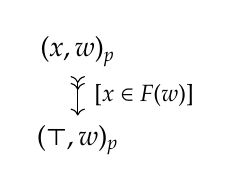
\begin{tikzpicture}[main/.style]
	\node[main] (1) {$(x, w)_p$};
	\node[main] (2) [below=0.5cm of 1] {$(\top, w)_{p}$};
	\draw[>>->] (1) -- (2) node[midway,sloped,right,rotate=90,scale=0.85] {\hspace{0.125cm}$[x\in F(w)]$};
	\end{tikzpicture}
	\caption{resolution of atomic formulas}
	\label{fig:atom_seq}
\end{figure}
If $x\notin F(w)$, then $\rightarrowdoubletail{}$ does not contain any move with $(x,w)_p$ as its first game state. The player $p$ cannot play a move, is stuck and loses. The game ends.\\
If $x\in F(w)$, then $\rightarrowdoubletail{}$ contains a single move $((x,w)_p,(\top,w)_p)$ with $(x,w)_p$ as its first game state. The player $p$ cannot play any other move and wins by reaching the winning position $(\top,w)_p\in E$. The game ends.
\end{itemize}
We show that the formula height is reduced by all other resolution sequences.
\begin{itemize}
\item Case $((\neg\varphi',w)_p, E, G, \rightarrowdoubletail{})$:\\
\begin{figure}[H]
	\centering
	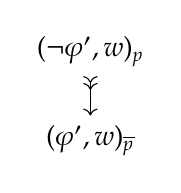
\begin{tikzpicture}[main/.style]
	\node[main] (1) {$(\neg\varphi', w)_p$};
	\node[main] (2) [below=0.5cm of 1] {$(\varphi', w)_{\overline{p}}$};
	\draw[>>->] (1) -- (2);
	\end{tikzpicture}
	\caption{resolution of negations}
	\label{fig:neg_seq}
\end{figure}
$\rightarrowdoubletail{}$ contains a single move $((\neg\varphi',w)_p,(\varphi',w)_{\overline{p}})$ with $(\neg\varphi',w)_p$ as its first game state. The player $p$ cannot play any other move and reduces the formula height by 1, because $h(\neg\varphi') = h(\varphi') + 1$.

\item Case $((\varphi'\vee\psi',w)_p, E, G, \rightarrowdoubletail{})$:\\
\begin{figure}[H]
	\centering
	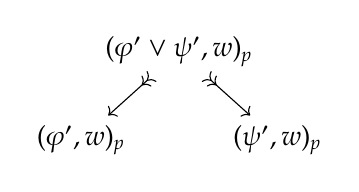
\begin{tikzpicture}[main/.style]
	\node[main] (1) {$(\varphi'\vee\psi', w)_p$};
	\node[main] (2) [below left=0.5cm and -0.5cm of 1] {$(\varphi', w)_{p}$};
	\node[main] (3) [below right=0.5cm and -0.5cm of 1] {$(\psi', w)_{p}$};
	\draw[>>->] (1) -- (2);
	\draw[>>->] (1) -- (3);
	\end{tikzpicture}
	\caption{resolution of disjunctions}
	\label{fig:disj_seq}
\end{figure}
$\rightarrowdoubletail{}$ contains two moves $((\varphi'\vee\psi',w)_p,(\varphi',w)_{p})$ and $((\varphi'\vee\psi',w)_p,(\psi',w)_{p})$ with the game state $(\varphi'\vee\psi',w)_p$ as their first member. The player $p$ can choose which move to play and reduces the formula height by 1 or more, because $h(\varphi'\vee\psi') = max(h(\varphi'),h(\psi')) + 1$.

\item Case $((\varphi'\wedge\psi',w)_p, E, G, \rightarrowdoubletail{})$:\\
\begin{figure}[H]
	\centering
	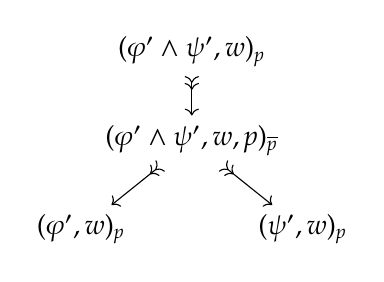
\begin{tikzpicture}[main/.style]
	\node[main] (1) {$(\varphi'\wedge\psi', w)_p$};
	\node[main] (2) [below=0.5cm of 1] {$(\varphi'\wedge\psi', w, p)_{\overline{p}}$};
	\node[main] (3) [below left=0.5cm and -0.5cm of 2] {$(\varphi', w)_{p}$};
	\node[main] (4) [below right=0.5cm and -0.5cm of 2] {$(\psi', w)_{p}$};
	\draw[>>->] (1) -- (2);
	\draw[>>->] (2) -- (3);
	\draw[>>->] (2) -- (4);
	\end{tikzpicture}
	\caption{resolution of conjunctions}
	\label{fig:conj_seq}
\end{figure}
$\rightarrowdoubletail{}$ contains a single move $((\varphi'\wedge\psi',w)_p,(\varphi'\wedge\psi',w,p)_{\overline{p}})$ with $(\varphi'\wedge\psi',w)_p$ as its first game state. The player $p$ cannot play any other move and does so. Then $\rightarrowdoubletail{}$ contains two moves $((\varphi'\wedge\psi',w,p)_{\overline{p}},(\varphi',w)_{p})$ and $((\varphi'\wedge\psi',w)_{\overline{p}},(\psi',w)_{p})$ with the game state $(\varphi'\wedge\psi',w,p)_{\overline{p}}$ as their first member. The player $\overline{p}$ chooses a move to play and reduces the formula height by 1 or more, because $h(\varphi'\wedge\psi') = max(h(\varphi'),h(\psi')) + 1$.

\item Case $((\Diamond\varphi',w)_p, E, G, \rightarrowdoubletail{})$:\\
\begin{figure}[H]
	\centering
	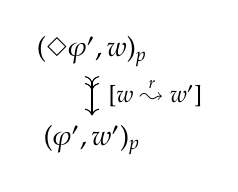
\begin{tikzpicture}[main/.style]
	\node[main] (1) {$(\Diamond\varphi',w)_p$};
	\node[main] (2) [below=0.5cm of 1] {$(\varphi', w')_{p}$};
	\draw[>>->] (1) -- (2) node[midway,sloped,right,rotate=90,scale=0.85] {\hspace{0.125cm}$[\smash{w\overset{r}{\leadsto}w'}]$};
	\end{tikzpicture}
	\caption{resolution of possibility}
	\label{fig:poss_seq}
\end{figure}
$\rightarrowdoubletail{}$ contains a move of the form $((\Diamond\varphi',w)_p,(\varphi',w')_{p})$ with $(\Diamond\varphi',w)_p$ as its first game state for each world $w'\in W_w$. The player $p$ can choose to play one of those moves and reduces the formula height by 1, because $h(\Diamond\varphi') = h(\varphi') + 1$.

\item Case $((\Box\varphi',w)_p, E, G, \rightarrowdoubletail{})$:\\
\begin{figure}[H]
	\centering
	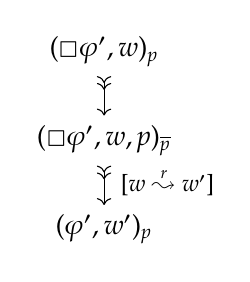
\begin{tikzpicture}[main/.style]
	\node[main] (1) {$(\Box\varphi',w)_p$};
	\node[main] (2) [below=0.5cm of 1] {$(\Box\varphi', w, p)_{\overline{p}}$};
	\node[main] (3) [below=0.5cm of 2] {$(\varphi', w')_{p}$};
	\draw[>>->] (1) -- (2);
	\draw[>>->] (2) -- (3) node[midway,sloped,right,rotate=90,scale=0.85] {\hspace{0.125cm}$[\smash{w\overset{r}{\leadsto}w'}]$};
	\end{tikzpicture}
	\caption{resolution of necessity}
	\label{fig:necc_seq}
\end{figure}
$\rightarrowdoubletail{}$ contains a single move $((\Box\varphi',w)_p,(\Box\varphi',w,p)_{\overline{p}})$ with $(\Box\varphi',w)_p$ as its first game state. The player $p$ cannot play any other move and does so. Then $\rightarrowdoubletail{}$ contains a move of the form $((\Box\varphi',w,p)_{\overline{p}},(\varphi',w')_{p})$ with $(\Box\varphi',w,p)_{\overline{p}}$ as its first game state for each world $w'\in W_w$. The player $\overline{p}$ can choose to play one of those moves and reduces the formula height by 1, because $h(\Box\varphi') = h(\varphi') + 1$.

\item Case $((\varphi'\Diamondright\psi',w)_p, E, G, \rightarrowdoubletail{})$:\\
\begin{figure}[H]
	\centering
	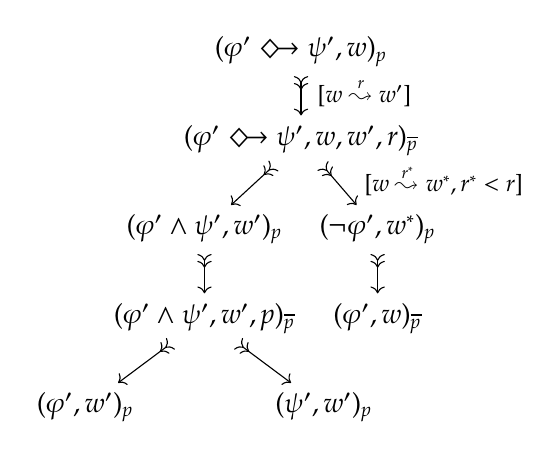
\begin{tikzpicture}[main/.style]
	\node[main] (1) {$(\varphi'\Diamondright\psi',w)_p$};
	\node[main] (2) [below=0.5cm of 1] {$(\varphi'\Diamondright\psi',w, w', r)_{\overline{p}}$};
	\node[main] (3) [below left=0.5cm and -1.5cm of 2] {$(\varphi'\wedge\psi', w')_{p}$};
	\node[main] (4) [below right=0.5cm and -1.5cm of 2] {$(\neg\varphi', w^*)_{p}$};
	
	\node[main] (5) [below=0.5cm of 3] {$(\varphi'\wedge\psi', w', p)_{\overline{p}}$};
	\node[main] (6) [below left=0.5cm and -0.5cm of 5] {$(\varphi', w')_{p}$};
	\node[main] (7) [below right=0.5cm and -0.5cm of 5] {$(\psi', w')_{p}$};
	
	\node[main] (8) [below=0.5cm of 4] {$(\varphi', w)_{\overline{p}}$};	
	
	\draw[>>->] (1) -- (2) node[midway,sloped,right,rotate=90,scale=0.85] {\hspace{0.125cm}$[\smash{w\overset{r}{\leadsto}w'}]$};
	\draw[>>->] (2) -- (3);
	\draw[>>->] (2) -- (4) node[midway,right,scale=0.85] {\hspace{0.25cm}$[\smash{w\overset{r^*}{\leadsto}w^*,r^*<r}]$};
	\draw[>>->] (3) -- (5);
	\draw[>>->] (5) -- (6);
	\draw[>>->] (5) -- (7);
	
	\draw[>>->] (4) -- (8);
	\end{tikzpicture}
	\caption{resolution of the counterfactual might}
	\label{fig:might_seq}
\end{figure}
$\rightarrowdoubletail{}$ contains a move of the form $((\varphi'\Diamondright\psi',w)_p,(\varphi'\Diamondright\psi',w,w',r)_{\overline{p}})$ with the game state $(\varphi'\Diamondright\psi',w)_p$ as its first member for each world $w'\in W_w$, $r\in [0,\infty ]$ and $\smash{w\overset{r}{\leadsto}w'}$. The player $p$ chooses to play one of those moves. Then $\rightarrowdoubletail{}$ contains a move of the form $((\varphi'\Diamondright\psi',w,w',r)_{\overline{p}},(\neg\varphi',w^*)_{p})$ with the game state $((\varphi'\Diamondright\psi',w,w',r)_{\overline{p}}$ as its first member for each $w^*\in W_{w,r}$ and also contains $((\varphi'\Diamondright\psi',w,w',r)_{\overline{p}},(\varphi'\wedge\psi',w')_{p})$.\\ If the player $\overline{p}$ chooses and plays one of the former moves, the formula height is reduced by 1, since $h(\varphi'\Diamondright\psi') = max(h(\varphi'),h(\psi')) + 1$. If the player $\overline{p}$ chooses and plays the latter and the player $p$ either plays resolves the resulting conjunction afterwards, then the formula height is reduced by 1, because $h(\varphi'\Diamondright\psi') = max(h(\varphi'),h(\psi')) + 1$.

\item Case $((\varphi'\boxright\psi',w)_p, E, G, \rightarrowdoubletail{})$:\\
\begin{figure}[H]
	\centering
	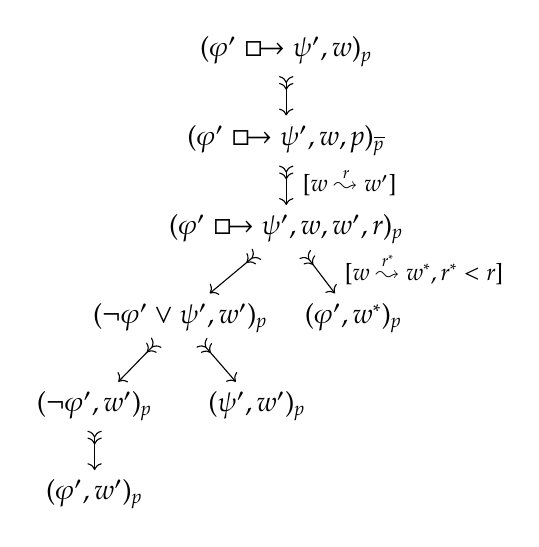
\begin{tikzpicture}[main/.style]
	\node[main] (0) {$(\varphi'\boxright\psi',w)_p$};
	\node[main] (1) [below=0.5cm of 0] {$(\varphi'\boxright\psi',w, p)_{\overline{p}}$};
	\node[main] (2) [below=0.5cm of 1] {$(\varphi'\boxright\psi',w, w', r)_{p}$};
	\node[main] (3) [below left=0.5cm and -1.5cm of 2] {$(\neg\varphi'\vee\psi', w')_{p}$};
	\node[main] (4) [below right=0.5cm and -1.5cm of 2] {$(\varphi', w^*)_{p}$};
	
	\node[main] (5) [below left=0.5cm and -1cm of 3] {$(\neg\varphi', w')_{p}$};
	\node[main] (6) [below right=0.5cm and -1cm of 3] {$(\psi', w')_{p}$};
	\node[main] (7) [below=0.5cm of 5] {$(\varphi', w')_{p}$};
	
	\draw[>>->] (0) -- (1);
	\draw[>>->] (1) -- (2) node[midway,sloped,right,rotate=90,scale=0.85] {\hspace{0.125cm}$[\smash{w\overset{r}{\leadsto}w'}]$};
	\draw[>>->] (2) -- (3);
	\draw[>>->] (2) -- (4) node[midway,right,scale=0.85] {\hspace{0.25cm}$[\smash{w\overset{r^*}{\leadsto}w^*,r^*<r}]$};
	\draw[>>->] (3) -- (5);
	\draw[>>->] (3) -- (6);
	\draw[>>->] (5) -- (7);	
	
	\end{tikzpicture}
	\caption{resolution of the counterfactual would}
	\label{fig:would_seq}
\end{figure}
$\rightarrowdoubletail{}$ contains a single move $((\varphi'\boxright\psi',w)_p,(\varphi'\boxright\psi',w,p)_{\overline{p}})$ with $(\varphi'\boxright\psi',w)_p$ as its first game state. The player $p$ cannot play any other move and does so. $\rightarrowdoubletail{}$ contains a move of the form $((\varphi'\boxright\psi',w,p)_{\overline{p}},(\varphi'\boxright\psi',w,w',r)_{p})$ with the game state $(\varphi'\boxright\psi',w,p)_{\overline{p}}$ as its first member for each world $w'\in W_w$, $r\in [0,\infty ]$ and $\smash{w\overset{r}{\leadsto}w'}$. The player $\overline{p}$ chooses to play one of those moves. Then $\rightarrowdoubletail{}$ contains a move of the form $((\varphi'\boxright\psi',w,w',r)_{p},(\varphi',w^*)_{p})$ with the game state $((\varphi'\boxright\psi',w,w',r)_{p}$ as its first member for each $w^*\in W_{w,r}$ and contains the move $((\varphi'\boxright\psi',w,w',r)_{p},(\neg\varphi'\vee\psi',w')_{p})$. If the player $p$ chooses and plays one of the former moves, the formula height is reduced by 1, since $h(\varphi'\boxright\psi') = max(h(\varphi'),h(\psi')) + 1$. If the player $\overline{p}$ chooses and plays the latter and subsequently resolves the resulting disjunction, then the formula height of the formula is reduced by 1, because $h(\varphi'\boxright\psi') = max(h(\varphi'),h(\psi')) + 1$.
\end{itemize}
Considering that all games with a counterfactual formula of formula height 1 end, every counterfactual formula has a formula height greater than 0 and every resolution sequence of a counterfactual operator reduces the height of the current formula of a game by 1, all semantic games end.
\end{proof}
Since a semantic game can only result in a victory for for either the defender or attacker, the semantic game of counterfactuals is decided. If every game ends and the game results in the victory of one player, then every game is won by one player.

\subsection{Correctness proof}
We will show through induction that the semantic game of counterfactuals is correct. More precisely, we will show that for each formula $\varphi$, world $w$ and counterfactual Kripke structure $S=(W,\leadsto ,F)$, the defending player has a winning strategy in the corresponding semantic game $\mathfrak{S}[\varphi ,w,S]$, if and only if $S,w\vDash\varphi$. Because the defender always begins a game $\mathfrak{S}[\varphi ,w,S]$ as the active player we will show that the player $p$ wins the game $\mathfrak{S}_p[\varphi ,w,S]$, iff $S,w\vDash\varphi$.
\begin{proof}We begin by showing 3 base cases.
\begin{itemize}
\item Base Case $\varphi=\top$:\\
$S,w\vDash\top$ is true and the respective semantic game is $\mathfrak{S}_p[\top ,w,S]=((\top ,w)_p, E, G, \rightarrowdoubletail{}
l)$. Since $(\top ,w)_p\in E$, it follows that the player $p$ wins the game with any strategy.
\item Base Case $\varphi=\bot$:\\
$S,w\vDash\bot$ is false and the semantic game is $\mathfrak{S}_p[\bot ,w,S]=((\bot ,w)_p, E, G, \rightarrowdoubletail{})$. There is no move in $\rightarrowdoubletail{}$ with $(\bot ,w)_p$ as its first element (see figure \ref{fig:limit_ass_moves}). That means no move can be played in this game state. The player $p$ is stuck and loses the game with any strategy.
\item Base Case $\varphi=x$ and $x\in Atoms$:\\
$S,w\vDash x$ is true iff $x\in F(w)$. And the semantic game is $\mathfrak{S}_p[x,w,S]=((x ,w)_p, E, G, \rightarrowdoubletail{})$. We show that the player $p$ has a winning strategy, iff $x\in F(w)$. Suppose $x\in F(w)$, then $\rightarrowdoubletail{}$ contains the move $((x ,w)_p, (\top ,w)_p)$ (see definition \ref{def:limit_ass_set_moves} and figure \ref{fig:moves} move \ref{eq:atom_move}). $((x ,w)_p, (\top ,w)_p)$ is a winning play for the player $p$. And any strategy mapping $(x ,w)_p$ to $((x ,w)_p, (\top ,w)_p)$ is a winning strategy for the player $p$. Suppose $x\notin F(w)$, then $\rightarrowdoubletail{}$ does not contain any move with $(x ,w)_p$ as its first element (see~def.\ref{def:limit_ass_set_moves}). That means no move can be played. The player $p$ is stuck and loses the game with any strategy.
\end{itemize}
Given the induction hypothesis that the player $p'$ wins the game $\mathfrak{S}_{p'}[\varphi' ,w,S]$, iff $S,w\vDash\varphi'$; and the player $p'$ wins the game $\mathfrak{S}_{p'}[\psi' ,w,S]$, iff $S,w\vDash\psi'$, we show for each composite formula that the player $p$ wins the game $\mathfrak{S}_p[\varphi ,w,S]$, iff $S,w\vDash\varphi$.
\begin{itemize}

\item Induction Step $\varphi=\neg\varphi'$:\\
$S,w\vDash\neg\varphi'$ is true iff $S,w\nvDash\varphi'$. And the game is $\mathfrak{S}_p[\neg\varphi',w,S]=((\neg\varphi' ,w)_p, E, G, \rightarrowdoubletail{})$. There is only a single move $((\neg\varphi' ,w)_p, (\varphi' ,w)_{\overline{p}})$ that has $(\neg\varphi' ,w)_p$ as its first element and that is contained within $\rightarrowdoubletail{}$ (see figure \ref{fig:limit_ass_moves}). For this reason, every play of the game $\mathfrak{S}_p[\neg\varphi',w,S]$ begins with the partial play $(\neg\varphi' ,w)_p(\varphi' ,w)_{\overline{p}}$. And given the induction hypothesis we know that the player $\overline{p}$ wins the game $\mathfrak{S}_{\overline{p}}[\varphi',w,S]=((\varphi' ,w)_{\overline{p}}, E, G, \rightarrowdoubletail{})$, iff $S,w\vDash\varphi'$. Since the player $p$ loses when the player $\overline{p}$ wins and the player $p$ wins when the player $\overline{p}$ loses, we know that the player $p$ wins, iff $S,w\nvDash\varphi'$.

\item Induction Step $\varphi=\varphi'\vee\psi'$:\\
$S,w\vDash\varphi'\vee\psi'$ is true, iff $(S,w\vDash\varphi'$ or $S,w\vDash\psi')$. And the corresponding game is $\mathfrak{S}_p[\varphi'\vee\psi',w,S]=((\varphi'\vee\psi' ,w)_p, E, G, \rightarrowdoubletail{})$. $\rightarrowdoubletail{}$ contains exactly the two moves $((\varphi'\vee\psi' ,w)_p,(\varphi' ,w)_p)$ and $((\varphi'\vee\psi' ,w)_p,(\psi' ,w)_p)$ that have $(\varphi'\vee\psi' ,w)_p$ as their first element. Given the induction hypothesis, the player $p$ has a winning strategy for the game $\mathfrak{S}_{p}[\varphi' ,w,S]$, iff $S,w\vDash\varphi'$; and further has a winning strategy for the game $\mathfrak{S}_{p}[\psi' ,w,S]$, iff $S,w\vDash\psi'$. Suppose $S,w\vDash\varphi'$, then the player $p's$ winning strategy for $\mathfrak{S}_{p}[\varphi' ,w,S]$ is also a winning strategy for $\mathfrak{S}_p[\varphi'\vee\psi',w,S]$, if it maps $(\varphi'\vee\psi' ,w)_p$ to $((\varphi'\vee\psi' ,w)_p,(\varphi' ,w)_p)$. And suppose $S,w\vDash\psi'$, then the player $p's$ winning strategy for $\mathfrak{S}_{p}[\psi' ,w,S]$ is also a winning strategy for $\mathfrak{S}_p[\varphi'\vee\psi',w,S]$, if it maps $(\varphi'\vee\psi' ,w)_p$ to $((\varphi'\vee\psi' ,w)_p,(\psi' ,w)_p)$. Lastly suppose $S,w\nvDash\varphi'$ and $S,w\nvDash\psi'$, then no winning strategy exists for the player $p$ and any of the games $\mathfrak{S}_{p}[\varphi' ,w,S]$ and $\mathfrak{S}_{p}[\psi' ,w,S]$. Because the player $p$ cannot make any move that does not transition into one of those two games, no winning strategy exists for the player $p$ and game $\mathfrak{S}_p[\varphi'\vee\psi',w,S]$.

\item Induction Step $\varphi=\varphi'\wedge\psi'$:\\
$S,w\vDash\varphi'\wedge\psi'$ is true, iff $(S,w\vDash\varphi'$ and $S,w\vDash\psi')$. And the corresponding game is $\mathfrak{S}_p[\varphi'\wedge\psi',w,S]=((\varphi'\wedge\psi' ,w)_p, E, G, \rightarrowdoubletail{})$. Every play of $\mathfrak{S}_p[\varphi'\wedge\psi',w,S]$ begins with either one of the following partial plays $(\varphi'\wedge\psi' ,w)_p(\varphi'\wedge\psi' ,w,p)_{\overline{p}}(\varphi' ,w)_p$ and $(\varphi'\wedge\psi' ,w)_p(\varphi'\wedge\psi' ,w,p)_{\overline{p}}(\varphi' ,w)_p$. Given the induction hypothesis, the player $p$ has a winning strategy for the game $\mathfrak{S}_{p}[\varphi' ,w,S]$, iff $S,w\vDash\varphi'$; and further has a winning strategy for the game $\mathfrak{S}_{p}[\psi' ,w,S]$, iff $S,w\vDash\psi'$. Suppose $S,w\nvDash\varphi'$, then the player $p$ loses the game $\mathfrak{S}_{p}[\varphi' ,w,S]$. In that case, any strategy that maps $(\varphi'\wedge\psi',w,p)_{\overline{p}}$ to $((\varphi'\wedge\psi' ,w,p)_{\overline{p}},(\varphi' ,w)_p)$ is a winning strategy for the player $\overline{p}$ and game $\mathfrak{S}_p[\varphi'\wedge\psi',w,S]$. Analogously suppose $S,w\nvDash\psi'$, then the player $p$ loses the game $\mathfrak{S}_{p}[\psi' ,w,S]$. In that case, any strategy that maps $(\varphi'\wedge\psi',w,p)_{\overline{p}}$ to $((\varphi'\wedge\psi' ,w,p)_{\overline{p}},(\psi' ,w)_p)$ is a winning strategy for the player $\overline{p}$ and game $\mathfrak{S}_p[\varphi'\wedge\psi',w,S]$. Lastly suppose $S,w\vDash\varphi'$ and $S,w\vDash\psi'$, then a winning strategy exists for the player $p$ and each of the games $\mathfrak{S}_{p}[\varphi' ,w,S]$ and $\mathfrak{S}_{p}[\psi' ,w,S]$. Because the player $\overline{p}$ cannot make any move that does not transition into one of those two games, no winning strategy exists for the player $\overline{p}$ and game $\mathfrak{S}_p[\varphi'\wedge\psi',w,S]$.

\item Induction Step $\varphi=\Diamond\varphi'$:\\
$S,w\vDash\Diamond\varphi'$ is true, iff a world $w'\in W_w$ exists, such that $S,w\vDash\varphi'$. And the semantic game is $\mathfrak{S}_p[\Diamond\varphi',w,S]=((\Diamond\varphi' ,w)_p, E, G, \rightarrowdoubletail{})$. Every play of $\mathfrak{S}_p[\Diamond\varphi',w,S]$ begins with a partial play of the form $(\Diamond\varphi' ,w)_p(\varphi' ,w')_p$ where $w'\in W_w$ ranges over the set of worlds $W_w$ that are accessible from $w$ (see definition \ref{def:limit_ass_set_moves} and figure \ref{fig:moves} move \ref{eq:poss_move}). Suppose there is an accessible world $w'\in W_w$, such that $S,w'\vDash\varphi'$. Then given the induction hypothesis, it is the case that the player~$p$ has a winning strategy for the corresponding game $\mathfrak{S}_{p}[\varphi' ,w',S]$. And if that strategy maps $(\Diamond\varphi' ,w)_p$ to $((\Diamond\varphi' ,w)_p,(\varphi' ,w')_p)$, it is also a winning strategy for the player $p$ and game $\mathfrak{S}_p[\Diamond\varphi',w,S]$. Conversely suppose there is no accessible world $w'\in W_w$, such that $S,w'\vDash\varphi'$. Then given the induction hypothesis, the player~$p$ does not have a winning strategy for any game of the form $\mathfrak{S}_{p}[\varphi' ,w',S]$ where $w'\in W_w$. But because every play of the game $\mathfrak{S}_p[\Diamond\varphi',w,S]$ begins with a partial play that transitions into a game of the form $\mathfrak{S}_{p}[\varphi' ,w',S]$ where $w'\in W_w$, the player $p$ loses the game $\mathfrak{S}_p[\Diamond\varphi',w,S]$.

\item Induction Step $\varphi=\Box\varphi'$:\\
$S,w\vDash\Box\varphi'$ is true, iff for every world $w'\in W_w$, it is true that $S,w\vDash\varphi'$. And the semantic game is $\mathfrak{S}_p[\Box\varphi',w,S]=((\Box\varphi' ,w)_p, E, G, \rightarrowdoubletail{})$. Every play of $\mathfrak{S}_p[\Box\varphi',w,S]$ begins with a partial play of the form $(\Box\varphi' ,w)_p(\Box\varphi' ,w,p)_{\overline{p}}(\varphi' ,w')_p$ where $w'\in W_w$ ranges over the set of worlds $W_w$ that are accessible from $w$ (see fig.\ref{fig:moves} moves \ref{eq:neccsw_move},\ref{eq:necc_move}). Suppose that there is an accessible world $w'\in W_w$, such that $S,w'\nvDash\varphi'$. Then given the induction hypothesis, the player $\overline{p}$ has a winning strategy for the game $\mathfrak{S}_p[\varphi',w',S]$. And if that strategy maps $(\Box\varphi' ,w,p)_{\overline{p}}$ to $((\Box\varphi' ,w,p)_{\overline{p}},(\varphi' ,w')_p)$, it is also a winning strategy for the player $\overline{p}$ and game $\mathfrak{S}_p[\Box\varphi',w,S]$. Conversely suppose that there is no accessible world $w'\in W_w$, such that $S,w'\nvDash\varphi'$. Then given the induction hypothesis, the player~$\overline{p}$ does not have a winning strategy for any game of the form $\mathfrak{S}_{p}[\varphi' ,w',S]$ where $w'\in W_w$. But because every play of the game $\mathfrak{S}_p[\Box\varphi',w,S]$ begins with a partial play that transitions into a game of the form $\mathfrak{S}_{p}[\varphi' ,w',S]$ where $w'\in W_w$, the player $\overline{p}$ loses the game $\mathfrak{S}_p[\Box\varphi',w,S]$ and $p$ wins.

\item Induction Step $\varphi=\varphi'\Diamondright\psi'$:\\
$S,w\vDash\varphi'\Diamondright\psi'$ is true, iff both a world $w'\in W_w$ with $S,w'\vDash\varphi'$ exists and for every world $w''$ and $r''$ for which $\smash{w\overset{r''}{\leadsto}w''}$ and $S,w'' \vDash \varphi\wedge\neg\psi$ are true, a world $w^*\in W_{w,r''}^\leq$ with $S,w^* \vDash \varphi\wedge\psi$ exists. And the corresponding semantic game is $\mathfrak{S}_p[\varphi'\Diamondright\psi',w,S]=((\varphi'\Diamondright\psi' ,w)_p, E, G, \rightarrowdoubletail{})$. Every play of the game $\mathfrak{S}_p[\varphi'\Diamondright\psi',w,S]$ begins with one of the two forms of partial plays $(\varphi'\Diamondright\psi' ,w)_p(\varphi'\Diamondright\psi' ,w,w',r)_{\overline{p}}(\varphi'\wedge\psi' ,w')_p$ and $(\varphi'\Diamondright\psi' ,w)_p(\varphi'\Diamondright\psi' ,w,w',r)_{\overline{p}}(\neg\varphi' ,w^*)_p$ where $w'\in W$; $w^*\in W_{w,r}^<$; $r\in [0,\infty ]$ and $\smash{w\overset{r}{\leadsto}w'}$ (see figure \ref{fig:limit_ass_moves} moves \ref{eq:limit_ass_mightsp_move},\ref{eq:limit_ass_mightde_move},\ref{eq:limit_ass_mightcl_move}).\\


Suppose no $\varphi'$-world is accessible from $w$. Then $S,w'\nvDash\varphi'$ for each world $w'\in W_w$. And given the induction hypothesis, the player $\overline{p}$ has a winning strategy for the game $\mathfrak{S}_p[\varphi',w',S]$. That strategy is also a winning strategy for the player $\overline{p}$ and game $\mathfrak{S}_p[\varphi'\Diamondright\psi',w,S]$, if it maps $(\varphi'\Diamondright\psi' ,w,w',r)_{\overline{p}}$ to $((\varphi'\Diamondright\psi' ,w,w',r)_{\overline{p}}, (\varphi'\wedge\psi' ,w')_p)$ and it maps $(\varphi'\wedge\psi' ,w,p)_{\overline{p}}$ to $((\varphi'\wedge\psi' ,w,p)_{\overline{p}}, (\varphi' ,w')_p)$. It follows that the player $\overline{p}$ wins the game $\mathfrak{S}_p[\varphi'\Diamondright\psi',w,S]$.\\

Now instead suppose that there exists at least one $\varphi'$-world that is accessible from~$w$. Applying the limit assumption, it follows that a $\varphi'$-world accessible from $w$ exists, such that no other $\varphi'$-world accessible from $w$ is more similar to $w$ than it. And if and only if such a world $w'\in W_w$ and an $r\in [0,\infty ]$ with $\smash{w\overset{r}{\leadsto}w'}$ and $S,w'\vDash\varphi'\wedge\psi'$~exist, such that no world $w^*\in W_{w,r}^<$ with $S,w^*\vDash\varphi'$ exists, then $w'$ is a world, such that for every world $w''\in W_w$ and $r''\in [0,\infty ]$ with $\smash{w\overset{r''}{\leadsto}w''}$ and $S,w''\vDash\varphi'\wedge\neg\psi'$, it holds that $r\leq r''$ and $\smash{w\overset{r}{\leadsto}w'}$ and $S,w'\vDash\varphi'\wedge\psi'$. Which means that whenever a ($\varphi'\wedge\psi'$)-world $w'$ accessible from $w$ exists, such that there is no $\varphi'$-world $w''$ accessible from $w$ that is more similar to the world $w$ than $w'$, it is true that $S,w\vDash\varphi'\Diamondright\psi'$. We thus show that the player $p$ wins the game $\mathfrak{S}_p[\varphi'\Diamondright\psi',w,S]$ whenever there is a ($\varphi'\wedge\psi'$)-world accessible from $w$, such that there is no $\varphi'$-world accessible from $w$ that is more similar to $w$ than it.\\

Suppose that a world $w'\in W$ and an $r\in [0,\infty ]$ with $\smash{w\overset{r}{\leadsto}w'}$ and $S,w'\vDash\varphi'\wedge\psi'$~exist, such that no world $w^*\in W_{w,r}^<$ with $S,w^*\vDash\varphi'$ exists. Given the induction hypothesis, the player $p$ has a winning strategy for the game $\mathfrak{S}_p[\varphi'\wedge\psi',w',S]$. And since there is no $\varphi'$-world that is more similar to $w$ than $w'$, the player $p$ also has a winning strategy for every game of the form $\mathfrak{S}_p[\neg\varphi',w^*,S]$ where $w^*\in W_{w,r}^<$. We can define a strategy in such a way---picking and choosing the mappings from the previously mentioned winning strategies---that it is a winning strategy for the player $p$ for both of the aforementioned forms of games. If that strategy also maps $(\varphi'\Diamondright\psi' ,w)_{p}$ to $((\varphi'\Diamondright\psi' ,w)_{p}, (\varphi'\Diamondright\psi' ,w,w',r)_{\overline{p}})$, then it is a winning strategy for the player $p$ and game $\mathfrak{S}_p[\varphi'\Diamondright\psi',w,S]$.\\

Finally suppose that a world $w^*\in W$ and $r^*\in [0,\infty ]$ with $\smash{w\overset{r^*}{\leadsto}w^*}$ and $S,w^*\vDash\varphi'$ exist, such that no world $w'\in W_{w,r^*}^\leq$ with $S,w'\vDash\varphi'\wedge\psi'$ exists. Then, given the induction hypothesis, it holds for each world $w'\in W_w$ and $r\in [0,\infty ]$ with $\smash{w\overset{r}{\leadsto}w'}$ that the player~$\overline{p}$ has a winning strategy for either the game $\mathfrak{S}_p[\varphi'\wedge\psi',w',S]$ or $\mathfrak{S}_p[\neg\varphi',w^*,S]$. Again we can construct a strategy by combining all of those winning strategies' essential mappings, such that the constructed strategy is a winning strategy with respect to each game that one of the aforementioned strategies is a winning strategy of. If that strategy then maps $(\varphi'\Diamondright\psi', w, w', r)_{\overline{p}}$ to $((\varphi'\Diamondright\psi', w, w', r)_{\overline{p}}, (\varphi'\wedge\psi', w')_p)$ iff the constructed strategy contains a winning strategy for the player $\overline{p}$ and game $\mathfrak{S}_p[\varphi'\wedge\psi',w',S]$; and otherwise maps $(\varphi'\Diamondright\psi', w, w', r)_{\overline{p}}$ to $((\varphi'\Diamondright\psi', w, w', r)_{\overline{p}}, (\neg\varphi', w^*)_p)$ for each $w'$, then it is also a winning strategy for the player $\overline{p}$ and game $\mathfrak{S}_p[\varphi'\Diamondright\psi',w,S]$.

\item Induction Step $\varphi=\varphi'\boxright\psi'$:\\
$S,w\vDash\varphi'\boxright\psi'$, iff either no world $w'\in W_w$ with $S,w'\vDash\varphi'$ exists or a world~$w'$ and an $r$ exist, such that $\smash{w\overset{r}{\leadsto} w'}$ and $S,w'\vDash\varphi'$ and for each world $w^*\in W_{w,r}^\leq$ it holds that $S,w^*\vDash\neg\varphi'\vee\psi'$. And the game is $\mathfrak{S}_p[\varphi'\boxright\psi',w,S]=((\varphi'\boxright\psi' ,w)_p, E, G, \rightarrowdoubletail{})$. Every play of the semantic game $\mathfrak{S}_p[\varphi'\boxright\psi',w,S]$ begins with one of the two forms of partial plays $(\varphi'\boxright\psi' ,w)_p(\varphi'\boxright\psi' ,w,p)_{\overline{p}}(\varphi'\boxright\psi' ,w,w',r)_{p}(\neg\varphi'\vee\psi' ,w')_p$ and $(\varphi'\boxright\psi' ,w)_p(\varphi'\boxright\psi' ,w,p)_{\overline{p}}(\varphi'\boxright\psi' ,w,w',r)_{p}(\varphi' ,w^*)_p$ where $w'\in W$; $w^*\in W_{w,r}^<$; $r\in [0,\infty ]$ and $\smash{w\overset{r}{\leadsto}w'}$ (see figure \ref{fig:limit_ass_moves} moves \ref{eq:limit_ass_wouldsw_move},\ref{eq:limit_ass_wouldsp_move},\ref{eq:limit_ass_wouldde_move},\ref{eq:limit_ass_wouldcl_move}).\\

Suppose no $\varphi'$-world is accessible from $w$. Then $S,w'\nvDash\varphi'$ for each world $w'\in W_w$. And given the induction hypothesis, the player $p$ has a winning strategy each game $\mathfrak{S}_{\overline{p}}[\varphi',w',S]$ with $w'\in W_w$. It follows that the player $p$ also has a winning strategy for each game $\mathfrak{S}_{p}[\neg\varphi',w',S]$ with $w'\in W_w$ and moreover has a winning strategy for each game $\mathfrak{S}_{p}[\neg\varphi'\vee\psi',w',S]$ with $w'\in W_w$. Those strategies can in turn be combined into one strategy that is a winning strategy for the player $p$ and every game of the form $\mathfrak{S}_{p}[\neg\varphi'\vee\psi',w',S]$ with $w'\in W_w$. If that strategy also maps every game state of the form $(\varphi'\boxright\psi' ,w,w',r)_{p}$ with $w'\in W_w$; $r\in [0,\infty ]$ and $\smash{w\overset{r}{\leadsto}w'}$ to $((\varphi'\boxright\psi' ,w,w',r)_{p},(\neg\varphi'\vee\psi' ,w')_p)$, then it also a winning strategy for the player $p$ and game $\mathfrak{S}_p[\varphi'\boxright\psi',w,S]$.\\

Now instead suppose that there exists at least one $\varphi'$-world that is accessible from~$w$. Applying the limit assumption, it follows that a $\varphi'$-world accessible from $w$ exists, such that no other $\varphi'$-world accessible from $w$ is more similar to $w$ than it. And if and only if it is the case that a $w'\in W$ and an $r\in [0,\infty ]$ with $\smash{w\overset{r}{\leadsto}w'}$ and $S,w'\vDash\varphi'\wedge\neg\psi'$~exist, such that no world $w^*\in W_{w,r}^<$ with $S,w^*\vDash\varphi'\wedge\psi'$ exists, then it holds that no world $w''\in W_w$ and $r''\in [0,\infty ]$ with $\smash{w\overset{r''}{\leadsto} w''}$ and $S,w''\vDash\varphi'$ exist, such that for each world $w^*\in W_{w,r}^\leq$ it holds that $S,w^*\vDash\neg\varphi'\vee\psi'$. Which means that whenever a ($\varphi'\wedge\neg\psi'$)-world $w'$ accessible from $w$ exists, such that there is no $\varphi'$-world $w^*$ accessible from $w$ that is more similar to the world $w$ than $w'$, it is true that $S,w\nvDash\varphi'\boxright\psi'$. We thus show that the player $p$ wins the game $\mathfrak{S}_p[\varphi'\boxright\psi',w,S]$ whenever there is no ($\varphi'\wedge\neg\psi'$)-world accessible from $w$, such that there is no $\varphi'$-world accessible from $w$ that is more similar to $w$ than it.\\

Suppose that a world $w^*\in W_w$ and an $r^*\in [0,\infty ]$ with $\smash{w\overset{r^*}{\leadsto}w^*}$ and $S,w^*\vDash\varphi'$ exist, such that no world $w'\in W_{w,r^*}^\leq$ with $S,w'\vDash\varphi'\wedge\neg\psi'$ exists. Then $w^*\vDash\varphi'\wedge\psi'$ and each world at least as similar to $w$ as $w^*$ is also a $(\neg\varphi'\vee\psi')$-world. Given the induction hypothesis, the player $p$ has a winning strategy for the game $\mathfrak{S}_p[\varphi'\wedge\psi',w^*,S]$. It follows that the player $p$ also has a winning strategy for the game $\mathfrak{S}_{p}[\psi',w^*,S]$ and moreover has a winning strategy for $\mathfrak{S}_{p}[\neg\varphi'\vee\psi',w^*,S]$. Given the induction hypothesis, it also holds that the player $p$ has a winning strategy for the game $\mathfrak{S}_p[\varphi',w^*,S]$. We can combine the latter two strategies into one strategy that is a winning strategy with respect to both the games $\mathfrak{S}_{p}[\neg\varphi'\vee\psi',w^*,S]$ and $\mathfrak{S}_p[\varphi',w^*,S]$. If that strategy also maps every game state of the form $(\varphi'\boxright\psi',w,w',r)_{p}$ with $w'\in W\setminus{}\{w^*\}$; $r\in [0, \infty ]$ and $\smash{w\overset{r}{\leadsto}w'}$ to $((\varphi'\boxright\psi',w,w',r)_{p}, (\varphi',w^*)_{p})$; and maps the game state $(\varphi'\boxright\psi',w,w^*,r^*)_{p}$ to $((\varphi'\boxright\psi',w,w^*,r^*)_{p},(\neg\varphi'\vee\psi',w^*)_{p})$, it is a winning strategy for the player $p$ and game $\mathfrak{S}_p[\varphi'\boxright\psi',w,S]$.\\


Suppose that a world $w'$ and an $r$ with $\smash{w\overset{r}{\leadsto}w'}$ and $S,w'\vDash\varphi'\wedge\neg\psi'$~exist, such that no world $w^*\in W_{w,r}^<$ with $S,w^*\vDash\varphi'$~exists. Then given the induction hypothesis, the player~$\overline{p}$ has a winning strategy for each game of the form $\mathfrak{S}_p[\varphi',w^*,S]$ where $w^*\in W_{w,r}^<$ and also has a winning strategy for the game $\mathfrak{S}_p[\neg\varphi'\vee\psi',w',S]$. Again we can construct a strategy that is a winning strategy for the player $\overline{p}$ with respect to each game of the form $\mathfrak{S}_p[\varphi',w^*,S]$ where $w^*\in W_{w,r}^<$ and also is a winning strategy for the player $\overline{p}$ and game $\mathfrak{S}_p[\neg\varphi'\vee\psi',w',S]$.
And if that strategy maps $(\varphi'\boxright\psi',w,p)_{\overline{p}}$ to $((\varphi'\boxright\psi',w,p)_{\overline{p}}, (\varphi'\boxright\psi',w,w',r)_{p})$, it is a winning strategy for the player $\overline{p}$ and game $\mathfrak{S}_p[\varphi'\boxright\psi',w,S]$.
\end{itemize}
\end{proof}

\section{The interactive demonstration}
This section introduces the interactive demonstration of the semantic game of counterfactuals and explores its presentation and correspondence to the semantic game. We will begin by explaining the game metaphor and offering an overview of the user interface. Afterwards, we will look in much greater detail at some parts of the web demonstration's visual presentation and explain user interaction and the process of playing the game. Then, we highlight some limitations of the web demonstration and differences to the semantic game. And finally, we discuss the algorithm that is used to compute a player's best move in a given game position.
\subsection{Game metaphor}
The semantic game's demonstration employs an embellishing metaphor for the course of the game in an effort to veil the complexity of the semantic game of counterfactuals and more succinctly convey its notions. The metaphor's most general sense is that the players are pilots of a spaceship that are tasked with traveling between possible worlds in order to reach a second earth. This interpretation lets Lewis' notion of the realism of possible worlds become palpable and provides an intuitive explanation for both players having the same current world, because they travel together. In order to discern the players, the metaphor uses the term pilot to describe the defender and copilot to describe the attacker, which also has a drawback. As most people tend to view the relationship between a pilot and copilot as one of collaboration and teamwork, it is not immediately obvious that the relationship between the pilot and copilot is adversarial in this case. The metaphor explains the adversity of the pilots by both of them wanting to be the first human to land on the second earth and figuratively make a small step for a man, but a giant leap for mankind. The act of landing is thus a metaphor for reaching the $\top$-symbol and winning the reachability game. The loss condition that a player that is stuck in turn is explained by that player being dismissed from their position as pilot for stranding the spaceship. Returning to our general metaphor we can explain the general makeup of a game state $(\varphi, w)_p$. The formula $\varphi$ is a schedule that the pilots have to strictly abide by. This schedule was precalculated by the boardcomputer, such that it is definitely possible to reach a habitable world by adhering to it. The world $w$ is merely the world the pilots' spaceship is currently at. And the active player $p$ is the pilot whose shift it currently is. The pilots work in shifts determined by the schedules shift switches that are metaphors for negations. Since different atomic formulas are true at different possible worlds, we call atomic formulas habitability tests. A world can only be landed on, if a habitability test was successfully conducted there. The possibility and necessity operators are simply jumps of the spaceship to another reachable world. And the counterfactual might and counterfactual would are explained as the opposing pilot's meddling with the board computer in order to temporarily limit the spaceships jump range.
\subsection{User interface \& interaction}
The game screen of the interactive demonstration appears as follows.
\begin{figure}[H]
\centering
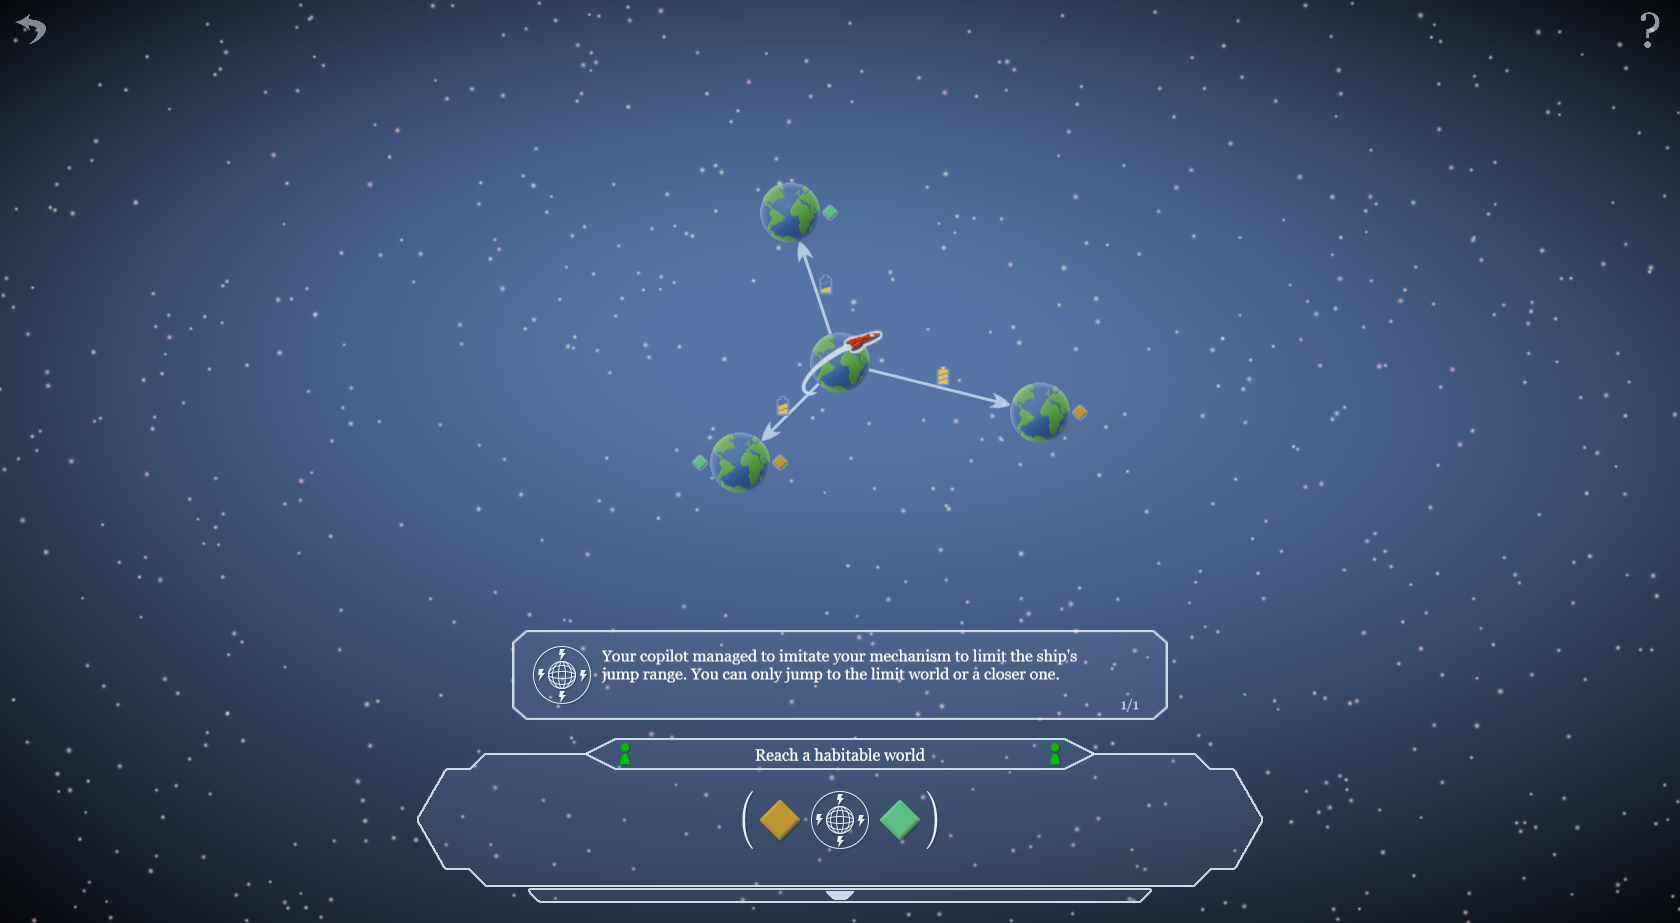
\includegraphics[width=\textwidth]{UI_Layout}
\caption{User interface}
\end{figure}
The center of the screen is taken up by a graph representation of a counterfactual Kripke structure. The similarity relation is represented through directed, labeled edges between possible worlds. Those edges are labeled with battery icons with 3 distinct charge states. The charge state of the battery is the value of the Kripke structure's respective measure of similarity between worlds. And for the sake of simplicity of this demonstration the similarity values are constrained to 4 values $0,1,2$ and $3$ in order of ascending dissimilarity. Reflexive edges are not displayed, but implicitly assumed to exist for each world and have a similarity value of 0. Additionally, the current world is indicated through a spaceship that is flying around a world. And small squares around the worlds visualize the distinct members of the set of atoms $F(w)$ of each world $w$. Every color corresponds to a different atomic formula.\\
\indent At the bottom of the screen there is a user interface element that we call the supposition panel. It holds a representation of the current formula and a prompt line that either describes what is currently happening or informs the user, if their input is required i.e. they have to make a choice. On the sides of the prompt line, there are icons that symbolize the active player. They are green if the defender---that is, user---is the active player and red otherwise.
There are also some other minor user interface elements like a textbox that introduces the game's rules, a back button and a help button with visualizations of the game's moves.\\
\indent The game automatically simulates all moves where the user does not have a choice and pauses in the converse case to prompt the user. The user either chooses between a left and right formula in the supposition panel or chooses a world of the counterfactual Kripke structure by clicking on it. The corresponding user interface elements become highlighted when clickable. With this, let us illustrate the depiction of counterfactual formulas.

\subsection{Representing counterfactual formulas}
The icons for each type of symbol of the counterfactual logic are shown in figure \ref{fig:icons}.
\begin{figure}[H]
\centering
\subfloat[$\bot$]{
\includegraphics{Tank_Empty}}
\subfloat[$\top$]{
\includegraphics{Flag}}
\subfloat[$x$]{
\includegraphics{Atom}}
\subfloat[$\neg$]{
\includegraphics{Negation}}
\subfloat[$\vee$]{
\includegraphics{OR_Wide}}\\
\subfloat[$\wedge$]{
\includegraphics{AND_Wide}}
\subfloat[$\Diamond$]{
\includegraphics{Possibility}}
\subfloat[$\Box$]{
\includegraphics{Necessity}}
\subfloat[$\Diamondright$]{
\includegraphics{Cf_Might}}
\subfloat[$\boxright$]{
\includegraphics{Cf_Would}}
\caption{Icon representations}
\label{fig:icons}
\end{figure}
As discussed earlier, the $\bot$ icon is meant to symbolize stranding the spaceship and the $\top$ icon landing on a habitable world. Since there are an infinite number of atomic formulas, we show a red icon of a habitability characteristic as a stand-in for all other possible colors the icon can take. The icon for the negation shows the switch of players in its metaphorical shift switch. The $\vee$ and $\wedge$ operators are most easily conveyed as natural language sentence connectives that combine different instructions. As for $\Diamond$ and $\Box$, we simply abstract both as a jump to another world where the active player's opponent overrides the destination in case of $\Box$. The icons for $\boxright$ and $\Diamondright$ visualize the choice of a sphere of accessibility as a circle around a world. They fail however to clearly indicate that a jump to another world will subsequently take place. One may also rightly criticize that due to their symmetric design, they do not show that the antecedent and consequent are treated differently in the following resolution.\\
\indent The icons are arranged the same way the symbols of counterfactual logic are in a well-formed counterfactual formula. Additionally, we sometimes display brackets to disambiguate the structure of the represented formula. The figure \ref{fig:icon_formulas} shows some examples.

\begin{figure}[H]
\centering

\subfloat[$\bot\vee x$]{
\scalebox{.75}{

\includegraphics{Tank_Empty}

\includegraphics{OR}

\includegraphics{Atom}}
}
\subfloat[$x\wedge\Box\top$]{
\scalebox{.75}{

\includegraphics{Atom}

\includegraphics{AND}

\includegraphics{Possibility}

\includegraphics{Flag}}
}\\
\subfloat[$\neg x\boxright (x\vee\bot)$]{
\scalebox{.75}{

\includegraphics{Negation}

\includegraphics{Atom}

\includegraphics{Cf_Would}

\includegraphics{BO_Thin}

\includegraphics{Atom}

\includegraphics{OR}

\includegraphics{Tank_Empty}

\includegraphics{BC_Thin}}
}
\caption{Representations of counterfactual formulas}
\label{fig:icon_formulas}
\end{figure}
\newpage%TODO: remove
\subsection{Employment of the limit assumption}\label{sec:limit_ass_just}
We formulated two semantic games of counterfactuals $\mathfrak{T}[\varphi ,w,S]$ and $\mathfrak{G}[\varphi ,w,S]$. While the former is the canonical formulation, playtesting revealed that it has a number of drawbacks that make it less suitable for the application in an educational game. If we compare the resolution of the counterfactual operators with respect to the two sets of moves $\rightarrowsingletail{}$~and~$\rightarrowdoubletail{}$, it becomes clear that the resolution sequences of the counterfactual operators are considerably more complex in the canonical formulation. Let us give the counterfactual would's resolution sequences as an example.
\begin{figure}[H]
\centering

\subfloat[With $\rightarrowsingletail{}$]{
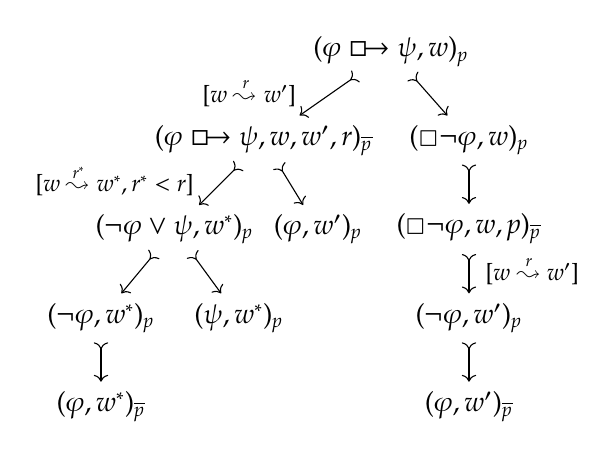
\begin{tikzpicture}[main/.style]
	\node[main] (0) {$(\varphi\boxright\psi,w)_p$};
	\node[main] (1) [below left=0.5cm and -1cm of 0] {$(\varphi\boxright\psi,w, w', r)_{\overline{p}}$};
	\node[main] (2) [below right=0.5cm and -1cm of 0] {$(\Box\neg\varphi,w)_{p}$};
	\node[main] (3) [below left=0.5cm and -1.5cm of 1] {$(\neg\varphi\vee\psi, w^*)_{p}$};
	\node[main] (4) [below right=0.5cm and -1.5cm of 1] {$(\varphi, w')_{p}$};
	\node[main] (5) [below=0.5cm of 2] {$(\Box\neg\varphi, w,p)_{\overline{p}}$};	
	\node[main] (6) [below left=0.5cm and -1cm of 3] {$(\neg\varphi, w^*)_{p}$};
	\node[main] (7) [below right=0.5cm and -1cm of 3] {$(\psi, w^*)_{p}$};
	\node[main] (8) [below=0.5cm of 5] {$(\neg\varphi, w')_{p}$};
	\node[main] (9) [below=0.5cm of 6] {$(\varphi, w^*)_{\overline{p}}$};
	\node[main] (10) [below=0.5cm of 8] {$(\varphi, w')_{\overline{p}}$};
	
	\draw[>->] (0) -- (1) node[midway,left,scale=0.85] {$[\smash{w\overset{r}{\leadsto}w'}]$\hspace{0.35cm} };
	\draw[>->] (0) -- (2);
	\draw[>->] (1) -- (3) node[midway,left,scale=0.85] {$[\smash{w\overset{r^*}{\leadsto}w^*,r^*<r}]$\hspace{0.25cm} };
	\draw[>->] (1) -- (4);
	\draw[>->] (2) -- (5);
	\draw[>->] (3) -- (6);
	\draw[>->] (3) -- (7);
	\draw[>->] (5) -- (8) node[midway,sloped,right,rotate=90,scale=0.85] {\hspace{0.125cm}$[\smash{w\overset{r}{\leadsto}w'}]$};
	\draw[>->] (6) -- (9);
	\draw[>->] (8) -- (10);
\end{tikzpicture}
}
\subfloat[With $\rightarrowdoubletail{}$]{
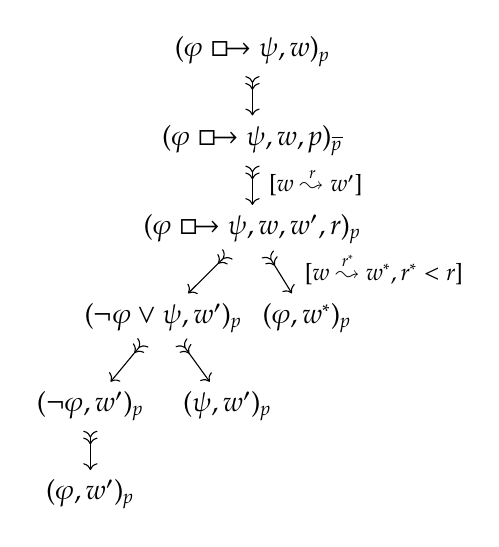
\begin{tikzpicture}[main/.style]
	\node[main] (0) {$(\varphi\boxright\psi,w)_p$};
	\node[main] (1) [below=0.5cm of 0] {$(\varphi\boxright\psi,w, p)_{\overline{p}}$};
	\node[main] (2) [below=0.5cm of 1] {$(\varphi\boxright\psi,w, w', r)_{p}$};
	\node[main] (3) [below left=0.5cm and -1.5cm of 2] {$(\neg\varphi\vee\psi, w')_{p}$};
	\node[main] (4) [below right=0.5cm and -1.5cm of 2] {$(\varphi, w^*)_{p}$};
	
	\node[main] (5) [below left=0.5cm and -1cm of 3] {$(\neg\varphi, w')_{p}$};
	\node[main] (6) [below right=0.5cm and -1cm of 3] {$(\psi, w')_{p}$};
	\node[main] (7) [below=0.5cm of 5] {$(\varphi, w')_{p}$};
	
	\draw[>>->] (0) -- (1);
	\draw[>>->] (1) -- (2) node[midway,sloped,right,rotate=90,scale=0.85] {\hspace{0.125cm}$[\smash{w\overset{r}{\leadsto}w'}]$};
	\draw[>>->] (2) -- (3);
	\draw[>>->] (2) -- (4) node[midway,right,scale=0.85] {\hspace{0.25cm}$[\smash{w\overset{r^*}{\leadsto}w^*,r^*<r}]$};
	\draw[>>->] (3) -- (5);
	\draw[>>->] (3) -- (6);
	\draw[>>->] (5) -- (7);	
\end{tikzpicture}
}
\caption{Resolution of the counterfactual would}
\label{fig:would_resolutions}
\end{figure}
We see that the players have to make more choices and consider more leaf states in~(a). For this reason, it becomes more difficult to introduce $\boxright$ and $\Diamondright$ in a digestible and understandable manner and convey them in simple terms. Since the user needs to understand the operators well in advance of play, this results in users being unable to take in the necessary information of a long-winded explanation. Furthermore, the structure of the counterfactual would's resolution under the canonical formulation of the semantic game requires a new dedicated paradigm of user interaction for claiming vacuous or non-vacuous truth that the users have to learn and understand as well. Such are the reasons that the interactive demonstration of counterfactuals adopts the game $\mathfrak{G}[\varphi ,w,S]$\footnote{As an improvement of user feedback the interactive demonstration differs from $\mathfrak{G}[\varphi ,w,S]$ in that players that are stuck transition to a game state with a $\bot$ formula and lose subsequently, and the attacker transitions to a $\top$ formula and switches the player when reaching a game state with the $\bot$ formula.}.

\subsection{Attacker move calculation}
In order to compute the attacker's most resilient continuations from a given game state, we developed a Minimax-algorithm that calculates a score for each reachable game state.
\begin{algorithm}[H]
\caption{Compute a score according to the function $sc$ for each reachable game position}\label{alg:minimax}
\begin{algorithmic}[1]
\Require $s$ (game state)
\Function{Scores}{$s$}\Comment{Score all possible game states}
	\State $Q \gets [s]$\Comment{Setup queue-, expanded node- and score lists}
	\State $E \gets []$
	\State $SC \gets []$
	\While{$Q$ not empty}
		\State $current \gets \Call{PEEK}{Q}$
		\State $e \gets \FALSE$
		\State $states \gets \Call{NEXTSTATES}{current}$
		\If{$current$ not in $E$}\Comment{Expand $current$}
			\State \Call{PUSH}{E, current}
			\State $e \gets \TRUE$
			\For{$s$ in $states$}
				\If{$s$ not in $E$}\Comment{Schedule $s$ for next expansion}
					\If{$s$ in $Q$}
						\State $\Call{REMOVEEACH}{$Q$, $s$}$
					\EndIf
					\State $\Call{PUSH}{$Q$, $state$}$
				\EndIf
			\EndFor
		\EndIf
		\If{e = \FALSE}\Comment{Process $current$, if it already has been expanded}
			\State $score \gets \Call{CALCSCORE}{current}$
			\State $\Call{PUSH}{$SC$, $score$}$
			\State $\Call{POP}{Q}$\Comment{Remove the processed element from $Q$}
		\EndIf
	\EndWhile
	\State \Return $SC$
\EndFunction
\end{algorithmic}
PEEK($Q$) retrieves the last element of the list $Q$, without removing it from $Q$\\
POP($Q$) retrieves the last element of the list $Q$ and removes it from $Q$\\
PUSH($Q$, $e$) appends an element $e$ to the end of the list $Q$\\
NEXTSTATES($s$) calculates the successor game states of the game state $s$\\
CALCSCORE($s$) calculates a score tuple for the game state $s$ according to $sc(s)$
\end{algorithm}
\begin{definition}[Score function]
Given that there are $n$ moves $m_{1, ..., n}$ with the game state $s$ as their first member and $sc(m_j)=(v_j, dec_j)$ for each $j\in\{1, ..., n\}$, we define the function $sc$.\\
If  $s=(\top,w)_a$ with $w\in W$ or the defender is stuck at $s$:\\
\begin{equation}
sc(s)=(0, 0)
\end{equation}
If  $s=(\top,w)_d$ with $w\in W$ or the attacker is stuck at $s$:\\
\begin{equation}
sc(s)=(1, 0)
\end{equation}
If $n>0$ and the defender is the active player at $s$:\\
\begin{equation}
sc(s)=((\Sigma^n_{i=1}v_{i})/n, (\Sigma^n_{i=1}dec_{i})/n+1)
\end{equation}
If $n>0$ and the attacker is the active player at $s$:\\
\begin{equation}
sc(s)=(v_{min}, dec_{min})\text{ where }v_{min}\leq v_i\text{ and }dec_{min}\leq dec_i\text{ for each }i\in\{1,...,n\}
\end{equation}
\end{definition}
The algorithm expands game state nodes like DFS, until it encounters a node that it has already expanded. In that case it processes that node and calculates our blunderscore metric for it. Since expanded nodes remain in the queue until they are processed, the queue can be intuited like a current path of search or processing order. Expanding a node is akin to considering all its dependencies and processing them first. It may happen, that a node that is already scheduled for processing (in the queue) is encountered another time. Then that node is deleted from the queue and pushed onto it (see lines 13-18). This means, simply that it is promoted to be processed earlier. And because the game graph does not contain cyclic dependencies, this does not run into infinite promotions of the processing order. In other words, because there are no cycles in the graph of game states, the algorithm will at some point encounter a node that has no successors and then be able to process it. If edges to the already processed nodes are left out of consideration, then there always is such a leaf node to process.

Since the AI in the game only ever calculates moves for the attacker, the definition of blunderscores is skewed that way. A converse formulation is easy to derive.

Alpha Beta cutoff is possible

\section{Results}
\bibliographystyle{alphaurl}
\nocite{*}
\bibliography{thesis}
\end{document}
